%% thesis.tex 2014/04/11
%
% Based on sample files of unknown authorship.
%
% The Current Maintainer of this work is Paul Vojta.

\documentclass{ucbthesis}
\usepackage{biblatex}

\usepackage{amssymb}
\usepackage{amsthm}
\usepackage{amsmath}
\usepackage{tikz}
\usepackage{tikz-cd}
\usepackage{mathrsfs}
\usepackage{url}


\usetikzlibrary{matrix}
\usetikzlibrary{decorations.markings}
\tikzset{
  closed/.style = {decoration = {markings, mark = at position 0.5 with { \node[transform shape, xscale = .7, yscale=.4] {/}; } }, postaction = {decorate} },
  open/.style = {decoration = {markings, mark = at position 0.5 with { \node[transform shape, scale = .7] {$\circ$}; } }, postaction = {decorate} }
}

\newtheorem{thm}{Theorem}[section]


\theoremstyle{definition}
\newtheorem{defn}[thm]{Definition}
\newtheorem{rmk}[thm]{Remark}
\newtheorem{exm}[thm]{Example}
\theoremstyle{theorem}
\newtheorem{lem}[thm]{Lemma}
\newtheorem{cor}[thm]{Corollary}
\newtheorem{prop}[thm]{Proposition}
\newtheorem{prob}[thm]{Exercise}


% To compile this file, run "latex thesis", then "biber thesis"
% (or "bibtex thesis", if the output from latex asks for that instead),
% and then "latex thesis" (without the quotes in each case).

% Double spacing, if you want it.  Do not use for the final copy.
% \def\dsp{\def\baselinestretch{2.0}\large\normalsize}
% \dsp

% If the Grad. Division insists that the first paragraph of a section
% be indented (like the others), then include this line:
% \usepackage{indentfirst}


\bibliography{references}

\begin{document}


\pagestyle{headings}

% (Optional) \part{First Part}

\include{chap1}
\include{chap2}
\include{chap3}

% \appendix


\chapter{Introduction}

The goal of this thesis is to give an exposition explaining Nicholas Katz's 2014 paper ``A Note on the Riemann Hypothesis for Hypersurfaces", where he gives a new proof of Deligne's classical result in the special case of hypersurfaces. The main result then is that the geometric zeta function of a smooth projective hypersurface $X/\mathbb{F}_q$ of dimension $d$ given by 

$$ Z(X,T) = exp(\sum\limits_{n=1}^{\infty}|X(\mathbb{F}_{q}^{n})|\frac{T^{n}}{n})$$

\noindent admits a factorization $\prod\limits_{i=0}^{2d}P_{i}^{(-1)^{i}}$, where $P_{i}$ is a $q$-Weil polynomial or weight $i$. While this result has been known in greater generality since the 70's, it's worth pointing out that the 2010 paper "Hypersurfaces and the Riemann Hypothesis" by A. Scholl reduced the general case of smooth proper varieties to that of hypersurfaces. The method of proof in that paper is a deformation argument, and does not use Lefschetz pencils or the $\ell$-adic Fourier transform. Thus, together with Scholl's paper this completes a new proof of the classical result.

As for the layout of the thesis, Chapter 2 of the thesis contains an in depth introduction to the tools needed to understand Katz's paper, some $\ell$-adic formalism, and an introduction to the Riemann hypothesis. It's fairly technical, so if the reader feels comfortable with the results they can check them as needed. Chapters 3 and 4 contain the main arguments presented in Katz's paper and are presented in more or less the same order as in the paper itself. Finally, there is an appendix presenting some ideas which were important, but tangential to the main discussion. I should point out that Katz's paper is itself only 10 pages, and can easily be found on his website if the reader prefers to read it in tandem with this thesis. 


The sketch of the main argument is roughly as follows. First we make some observations about the convergence of $L$-functions of so called $\iota$-real local systems on affine curves, which has direct applications to deducing purity for such local systems. The general result is theorem 3.2.5 which says that  weight $0$ purity of an $\iota$-real local system on an affine curve can be detected from a single closed point. After studying some general properties of the \'{e}tale cohomology groups of smooth hypersurfaces, we show that the Riemann hypothesis for an $n$ dimensional smooth hypersurface $X_{0,0}/\mathbb{F}_{q}$ of degree $d$ is equivalent to proving purity for the middle cohomology group $H^{n}(X_{0},\mathbb{Q}_{\ell})$ where $X_{0}$ is the base change of $X_{0,0}$ to $\overline{\mathbb{F}}_{q}$. Smooth and proper base change allows us to study this cohomology group in 1-parameter family $\{X_{t,0}\}$, which we then exploit in theorem 3.3.3 the following way. If $X_{1,0}/\mathbb{F}_{q}$ is another smooth hypersurface of dimension $n$ and degree $d$ for which it is known that $H^{n}(X_{1},\mathbb{Q}_{\ell})$ is pure of weight $n$, connect $X_{0,0}$ and $X_{1,0}$ in a fibration over the affine line over $\mathbb{F}_{q}$.  This fibration will be smooth over some open set $U_{0}$ containing the points $t=0,1$. Then by the assumption on $X_{1,0}$, if $\bar{u}_{1}$ is a geometric point above the point $t=1$ then the eigenvalues of $Frob_{t=1}|R^{n}f_{*}\mathbb{Q}_{\ell}(n/2)_{\bar{u}_{1}}$ are all of absolute value $1$. Together with our results on purity of local systems on curves this implies that $R^{n}f_{*}\mathbb{Q}_{\ell}$ is pure of weight $n$ on $U_{0}$, which proves the Riemann hypothesis for each fibre over $U_{0}$ and in particular for $X_{0}$. It then remains to find a smooth model of a hypersurface of dimension $n$ and degree $d$ over $\mathbb{F}_{p}$  satisfying the Riemann hypothesis for every triple $(n,d,p)$. We simplify the problem in corollary 3.2.5 by proving the classical result that in the case of hypersurfaces, the Riemann hypothesis is actually equivalent to a certain point counting formula. After treating a few individual cases, we then show that a certain hypersurface called Gabber's hypersurface satisfies the point counting formula for the rest of the cases. This is done in chapter 4 using Gauss sums and some elementary results from the theory of diagonalizable group schemes. 


I would like to thank my professors from Milan and Paris for everything they did for me in the last two years. I would also like to thank my adviser Tam\'{a}s Szamuely for suggesting the topic and helping me throughout the writing and editing process, as well as my adviser in Paris, David Harari.

\chapter{Introduction to the Riemann Hypothesis}

\section{Zeta Functions}
Let $X$ be a scheme of finite type over $\mathbb{F}_{q}$ where $q=p^{r}$ and let $|X|$ denote the set of closed points of $X$. The \textbf{zeta function} of $X$ is defined to be the complex valued function
$$\zeta(X,s) = \prod\limits_{x\in |X|}{\frac{1}{1-\mathbb{N}(x)^{-s}}}$$
where $\mathbb{N}(x)$ is the \textbf{norm} of $x$, which is by definition the size of the residue field $k(x)$. We define the \textbf{degree} of $x$ be $deg(x) = [k(x):\mathbb{F}_{q}]$. By the Nullstellensatz the degree and hence the norm of a closed point are finite. It's not difficult to show that $\zeta(X,s)$ converges uniformly on compact sets on the domain $\Re(s)>dim(X)$, where it defines a holomorphic function. Thus we can speak about the zeta function as an analytic object, about its singularities and zeros etc. 

Note that $deg(x)|n$ if and only if there exists a morphism $i:Spec(\mathbb{F}_{q^{n}})\rightarrow X$ over $Spec(\mathbb{F}_{q})$ with image $x$, i.e. an $\mathbb{F}_{q}$-homomorphism $k(x)\rightarrow \mathbb{F}_{q^{n}}$. In this case we say that $x$ is defined over $\mathbb{F}_{q^n}$, and that $i$ is an $\mathbb{F}_{q^{n}}$\textbf{-point} of $X$. This distinction between "points" in the sense of closed points of $X$ as a topological space and $\mathbb{F}_{q^{n}}$-points for some $n$ plays an important role. For example, take a closed point $x\in |X|$ with degree $d$, which then gives us a morphism $Spec(\mathbb{F}_{q^d}) \rightarrow X$. Precomposition with any nontrivial automorphism of $Spec(\mathbb{F}_{q^d})$ over $\mathbb{F}_{q}$ gives us a different $\mathbb{F}_{q^d}$-point with image $x$. As $\mathbb{F}_{q^{d}}/\mathbb{F}_{q}$ is separable, there are exactly $deg(x)$ such points with image $x$. In general we denote the set of all $\mathbb{F}_{q^{n}}$-points of $X$ by $X(\mathbb{F}_{q^n})$. We then have the following easy proposition:

\begin{prop}
\begin{enumerate}
  \item For any closed point $x$, the norm of $x$ is finite and a power of $q$.
  \item There are only finitely many points of a given norm, hence also of a given degree.  
  \item $|X(\mathbb{F}_{q^n})| = \sum\limits_{deg(x)|n}deg(x)$
\end{enumerate}
\end{prop}

\begin{proof}
\begin{enumerate}
  \item Obvious.
  \item We may cover $X$ by finitely many open subsets of the form $Spec(\mathbb{F}_{q}[x_1,\ldots,x_{n}]/I)$ where $I$ is generated by finitely many polynomials in the $x_{i}$. For a closed point $x$ in such an open set, $\mathbb{N}(x)\vert q^d$ if and only if $x$ corresponds to an $n$-tuple in $\mathbb{F}_{q^d}^n$ satisfying the equations in $I$. Certainly the number of such points is at most $(q^{d})^n$, hence the claim. 
  \item $|X(\mathbb{F}_{q^n})| = |\coprod\limits_{x\in |X|}Hom_{\mathbb{F}_{q}}(k(x),\mathbb{F}_{q^n})|= |\coprod\limits_{deg(x)|n}Hom_{\mathbb{F}_{q}}(k(x),\mathbb{F}_{q^n})| \vspace{5mm}\\ = \sum\limits_{deg(x)|n}|Hom_{\mathbb{F}_{q}}(k(x),\mathbb{F}_{q^n})| = \sum\limits_{deg(x)|n}deg(x).$
\end{enumerate} 
\end{proof}

We define the \textbf{geometric zeta function} of $X$ to be
$$Z(X,T) = exp(\sum\limits_{n=1}^{\infty}|X(\mathbb{F}_{q^n})|\frac{T^{n}}{n})$$

\begin{prop}
$Z(X,q^{-s}) = \zeta(X,s)$ whenever this equation makes sense.
\end{prop}
\begin{proof} Ignoring any questions of convergence we have that\\
$log(\zeta(X,s)) = \sum\limits_{x\in |X|}-log(1-N(x)^{-s}) = \sum\limits_{x\in |X|}\sum\limits_{n=1}^{\infty}\frac{N(x)^{-sn}}{n} = \sum\limits_{n=1}^{\infty}\sum\limits_{x\in |X|}\frac{N(x)^{-sn}}{n}\\ \vspace{.5mm} = \sum\limits_{n=1}^{\infty}\sum\limits_{x\in |X|}\frac{q^{-sn\cdot deg(x)}}{n} = \sum\limits_{m=1}^{\infty}(\sum\limits_{deg(x)|m}deg(x))\frac{q^{-sm}}{m}$\\
where the last equality follows from the substitution $m=n\cdot deg(x)$. By the previous proposition, $|X(\mathbb{F}_{q^n})_{\mathbb{F}_q}| = \sum_{deg(x)|n}deg(x)$, so making the substitution and taking exponentials gives the desired result. 
\end{proof}

\begin{defn} A \textbf{$q$-Weil number of weight $n$}$\in\mathbb{N}$ is an algebraic number for which all archemedian absolute values are $q^{n/2}$. A \textbf{$q$-Weil polynomial pure of weight $n$} is a polynomial $P$ with integer coefficients and constant term $1$ whose factorization\\ $P = \prod(1-\gamma_{j}T)$ has the property that all the $\gamma_{j}$ are $q$-Weil numbers of weight $n$.
\end{defn}

Assume further that $X$ is smooth, proper, geometrically connected and of pure dimension $d$. Then the \textbf{Riemann hypothesis} for $X$ is the following

\begin{thm}[\textbf{Riemann hypothesis}]
$Z(X,T) = \prod\limits_{0}^{2d}P_{i}(T)^{(-1)^{i+1}}$ where the polynomial $P_{i}$ is a $q$-Weil polynomial of weight $i$
\end{thm}

The goal of the next sections is to place the theory of zeta functions in a more general context where we will give a new interpretation of the Riemann hypothesis in terms of \'{e}tale cohomology. Ultimately we will be concerned only in the case of $X$ a hypersurface, and we will see how the study of the zeta function reduces to counting points defined over various extensions of $\mathbb{F}_{q}$. This technique is perhaps already foreshadowed by our discussion of the geometric zeta function, but we will see how further reductions allow us to solve the Riemann hypothesis by explicit point counting in a few concrete cases. 

\section{The Frobenius morphism}
There is one advantage that we inherit for free by working in characteristic $p$, namely the Frobenius morphism. It turns out there are several flavors of the Frobenius, but we begin by exploring some of the basic and important properties of the absolute Frobenius. It will play a decisive role in all that follows.  Here we will follow  [SGA 5 Exp. V 15].

Let $X$ be a scheme over $\mathbb{F}_{q}$. The (absolute) Frobenius endomorphism $fr_{X}:X \rightarrow X$ is defined to be the identity on the topological space, with $\mathcal{O}_{X} \rightarrow \mathcal{O}_{X}$ given by $f \mapsto f^{q}$. If $g:Y\rightarrow X$ is a morphism, it is a simple exercise to check that 
\begin{center}
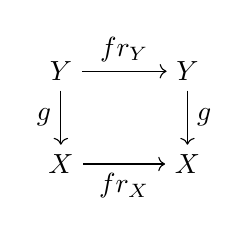
\begin{tikzpicture}
  \matrix (m) [matrix of math nodes,row sep=2em,column sep=3em,minimum width=1em]
   {Y & Y \\
   X & X\\};
  \path[->]
    (m-1-1) edge node[above]{$fr_{Y}$} (m-1-2);
  \path[->]
    (m-1-1) edge node[left]{$g$} (m-2-1);
  \path[->] 
    (m-1-2) edge node[right]{$g$} (m-2-2);
  \path[->] 
    (m-2-1) edge node[below]{$fr_{X}$}(m-2-2);
\end{tikzpicture}
\end{center}
is a commutative diagram, and in fact fixing $g$ and $fr_{X}$ in the diagram above, $fr_{Y}$ is the unique endomorphism of $Y$ making the diagram commute. Thus $fr_{X}$ depends functorially on $X$, or in categorical language that $fr_{\cdot}$ is an endomorphism of the identity transformation on $\mathbf{Sch}/\mathbb{F}_{p}$. 

It then follows that we have the cartesian diagram
\begin{center}
\begin{tikzcd}
Y \arrow[bend left]{drr}{fr_{Y}}
\arrow[bend right]{ddr}{g}
\arrow[dotted]{dr}[description]{Fr_{Y/X}} & & \\
& X \times_X Y \arrow{r}{\pi_{Y/X}} \arrow{d}{g^{(p)}} & Y \arrow{d}{g} \\
& X \arrow{r}{fr_{X}} & X
\end{tikzcd}
\end{center}

Denote the product $X\times_{X} Y$ in this diagram by $Y^{(p/X)}$. It's clear the assignment $p_{Y}:Y \leadsto Y^{(p/X)}$ is functorial in $Y$ since this is functor is just base change by $fr_{X}:X\rightarrow X$. We define the morphism $Fr_{Y/X}:Y \rightarrow Y^{(p/X)}$ to be the \textbf{relative Frobenius} of $Y$ relative to $X$. We have the following proposition concerning the relative Frobenius:

\begin{prop}
\begin{enumerate}
  \item $Fr_{\cdot/X}$ commutes with base change, i.e. if $f:X'\rightarrow X$ and $'$ denotes the base
   change functor relative to $X'$, then with the notation above we have $(Y^{(p/X)})'\simeq (Y')^{(p/X')}$ and $(Fr_{Y/X})' = Fr_{Y'/X'}$.
  \item $Fr_{Y/X}$ is functorial in $Y$ in the sense that if $g':Y'\rightarrow X$ is a morphism and $h:Y'\rightarrow Y$ is an $X$-morphism, then we have the following commutative diagram:
\begin{center}
\begin{tikzcd}
Y' \arrow{r}{Fr_{Y'/X}} \arrow{d}{h} & Y^{'(p/X)} \arrow{d}{h^p} \\
Y \arrow{r}{Fr_{Y/X}} \arrow{r} & Y^{(p/X)}
\end{tikzcd}
\end{center}
where the right vertical arrow is induced by base change. 
  \item The relative Frobenius $Fr_{Y/X}:Y\rightarrow Y^{(p/X)}$ is a universal homeomorphism, i.e. is a homeomorphism and remains so after base change. 
\end{enumerate}
\end{prop}

\begin{proof}
The proofs of the first two statements are formal. For the third statement, notice that by the base change properties in part one it suffices to show that $Fr_{Y/X}:Y\rightarrow Y^{p/X}$ is a homeomorphism. For this we use the following commutative diagram together with the fact that $fr_{Y}$ is the identity on topological spaces:
\begin{center}
\begin{tikzcd}
Y\arrow[bend left]{drr}[description]{fr_{Y}}
\arrow[bend right]{ddr}{g}
\arrow[dotted]{dr}[description]{Fr_{Y/X}} & & & 
Y^{(p/X)}\arrow[bend left]{ddl}{g^{(p)}}\\
& Y^{(p/X)} \arrow{r}{\pi_{Y/X}} \arrow{d}{g^{(p)}}\arrow[bend left]{urr}[description]{fr_{Y^{(p/X)}}} & Y \arrow{ur}[description]{Fr_{Y/X}} \arrow{d}{g}

\\
& X \arrow{r}{fr_{X}} & X
\end{tikzcd}
\end{center}
\end{proof}

\begin{cor}
$fr_{X}$ is a universal homeomorphism.
\end{cor}
\begin{proof}
With the above notation we want that $\pi_{Y/X}$ is a homeomorphism. This follows from the fact that $Fr_{Y/X}$ and $fr_{Y}$ are both homeomorphisms. 
\end{proof}


\begin{cor}
If $g:Y\rightarrow X$ is \'{e}tale, then $Fr_{Y/X}$ is an isomorphism. Hence together with proposition 2.2.1, $Fr_{\cdot/X}$ is natural isomorphism of the identity functor $id_{\mathbf{Sch/X}}$ and the base change functor $p:\mathbf{Sch/X} \rightarrow \mathbf{Sch/X}$ given by the Frobenius.
\end{cor}
\begin{proof}
More generally it holds that a universal homeomorphism $g:S \rightarrow T$ which is \'{e}tale is an isomorphism. For a proof of this fact see [Stacks tag 025F]. Ultimately we only care about the case when $X$ is a variety over $\mathbb{F}_{q}$, so we treat this case. We already know that $Fr_{Y/X}$ is a homeomorphism, so it remains to check that $Fr_{Y/X}^{\#}:\mathcal{O}_{X} \rightarrow (Fr_{Y/X})_{*}\mathcal{O}_{Y}$ is an isomorphism. One checks immediately that that in the case of varieties $Fr_{Y/X}$ is a finite \'{e}tale morphism, so $(Fr_{Y/X})_{*}\mathcal{O}_{Y}$ is a coherent $\mathcal{O}_{X}$-module, and that each induced morphism of residue fields is a separable extension. However they are also purely inseparable, since $Fr_{Y/X}$ is a universal homeomorphism hence radicielle. This implies that the maps of residue fields are all isomorphisms, so Nakayama's lemma implies the isomorphism. 
\end{proof}

Now let $\mathcal{F}$ be a sheaf on $X_{\acute{e}t}$, and consider the pushforward $fr_{S*}\mathcal{F}$ of $\mathcal{F}$
 by $fr_{X}$. By definition, for $U\rightarrow X$ \'{e}tale we have $fr_{X*}\mathcal{F}(U) = \mathcal{F}(U\times_{X}X)$,
  which using the above notation we rewrite as $F(U^{(p/S)})$. Then $\mathcal{F}(Fr_{U/S}^{-1}): \mathcal{F}(U) \rightarrow
   fr_{X*}\mathcal{F}(U)$ is an isomorphism functorial in $U$ by corollary 2.2.3, so we have constructed an isomorphism $\mathcal{F}
    \rightarrow fr_{X*}\mathcal{F}$. By adjunction this gives us an isomorphism\footnote{It's not obvious that the morphism given by the adjunction is also an isomorphism. However, we showed above that $fr_{X}$ is a universal homeomorphism, and it follows that the corresponding morphisms $fr_{X*}$ and $fr_{X}^{*}$ are mutually quasi-inverse. Thus isomorphisms map to isomorphisms.}
$Fr_{\mathcal{F}/X}^{*}:fr_{X}^{*}\mathcal{F} \rightarrow \mathcal{F}$. 

\begin{defn}
For a scheme $X$ defined over $\mathbb{F}_{q}$, and a sheaf $\mathcal{F}\in Sh(X_{\acute{e}t})$, we define the \textbf{Frobenius correspondence on $(X,\mathcal{F})$} to be the data $(fr_{X}$,$Fr_{\mathcal{F}/X})$ where $fr_{X}$ is the absolute Frobenius of $X$ and $Fr_{\mathcal{F}/X}: fr_{X}^{*}\mathcal{F} \rightarrow \mathcal{F}$ is the isomorphism described above. 
\end{defn}

We note that the Frobenius correspondence is functorial in $\mathcal{F}$, meaning that $Fr_{\cdot/X} :fr_{X}^{*} \rightarrow id_{Sh(X_{\acute{e}t})}$ is a natural isomorphism of functors. There is also a way to assign meaning to the phrase "the Frobenius correspondence is functorial in $X$" in the language of fibred categories, namely if $\mathcal{C}$ is the fibred category of \'e{t}ale sheaves over the category of schemes over $\mathbb{F}_{q}$, then the collection of $Fr_{\mathcal{F}/X}$ form an isomorphism of functors of fibred categories $fr_{*}\rightarrow id_{\mathcal{C}}$. We don't really need this, but it's interesting to note that the Frobenius correspondence is the unique such isomorphism. For details see [SGA 5 Exp. XV 2.1.1].  

\section{The \'{E}tale Fundamental Group}

Here we give a brief summary of basic results in the theory of \'{e}tale fundamental groups, going as far as the homotopy sequence and the correspondence between \'{e}tale covers and finite continuous $\pi_{1}$-sets.
For a more thorough treatment, see the standard references: [Szamuely ch. 5] or [SGA 1].

Let $X$ be a connected scheme. Then we consider the category $\mathcal{C}$ whose objects are schemes $Y$ over $X$ whose structure morphism to $X$ is finite \'{e}tale. We also call such a $Y/X$ a \textbf{finite \'{e}tale covering}. Fixing a geometric point $\bar{x}:Spec(\Omega)\rightarrow X$ with $\Omega$ a separably closed field, we can define the fibre functor $Fib_{\bar{x}}:\mathcal{C}\rightarrow \mathbf{FSet}$ which takes $Y\rightarrow X$ to the underlying finite set of $Y\times_{X}Spec(\Omega) = Y(\bar{x})$. We define the \textbf{\'{e}tale fundamental group} $\pi_{1}(X,\bar{x})$ to be the automorphism group of this functor, i.e. the group of all natural transformations $\eta:Fib_{\bar{x}}\rightarrow Fib_{\bar{x}}$ admitting a two sided inverse. We have the following results regarding the structure of $\pi_{1}(X,\bar{x})$:

\begin{prop}
\begin{enumerate}
 \item The fibre functor $Fib_{\bar{x}}$ is pro-representable by the inverse system of connected Galois covers\footnote{Remember that a finite \'{e}tale cover $Y\rightarrow X$ is said to be \textbf{Galois} if the automorphism group $Aut(Y|X)$ acts transitively on the geometric fibres $Y(\bar{x})$.} $(P_{\alpha},\phi_{\alpha,\beta})$, i.e. there is an isomorphism natural in $Y$: 
\begin{center}
$\varinjlim Hom_{X}(P_{\alpha},Y) \simeq Fib_{\bar{x}}(Y)$.
\end{center} 
\item Keeping the same notation, every automorphism of the fibre functor $Fib_{\bar{x}}$ comes from a unique automorphism of the inverse system $(P_{\alpha},\phi_{\alpha,\beta})$.
\item There is an isomorphism $\pi_{1}(X,\bar{x}) \simeq \varprojlim Aut(P_\alpha)^{opp}$
\end{enumerate}
\end{prop}

\begin{thm}
\begin{enumerate}
\item $\pi_{1}(X,\bar{x})$ is profinite, and its action on $Fib_{\bar{x}}(Y)$ is continuous for all $Y\in$Ob$(\mathcal{C})$. 
\item If $\bar{z}\rightarrow X$ is another geometric point, there is a natural isomorphism of functors
 $\gamma: Fib_{\bar{x}} \simeq Fib_{\bar{z}}$ inducing a continuous isomorphism $f_{\gamma}:\pi_{1}(X,\bar{x})
  \simeq \pi_{1}(X,\bar{z})$. Furthermore, if $f_{\gamma'}$ is another such isomorphism of fibre functors, then
   $f_{\gamma} = f_{\gamma'}$ up to composition with an inner automorphism of $\pi_{1}(X,\bar{x})$ or
    $\pi_{1}(X,\bar{z})$. 
\item The fibre functor $Fib_{\bar{x}}$ induces an equivalence of categories between $\mathcal{C}$ and the category of finite sets with a continuous $\pi_{1}(X,\bar{x})$ action. Moreover, under the connected Galois covers correspond to the finite $\pi_{1}(X,\bar{x})$-sets with a transitive action.
\end{enumerate} 
\end{thm}

\begin{exm} If $k$ is a field with separable closure $k^{s}$, then $\pi_{1}(Spec(k),Spec(k^{s})) = Gal(k^{s}/k)$.\end{exm}

Let $X'\xrightarrow{f} X$ be a morphism of connected schemes. Since the the property of being finite \'{e}tale is closed under base change, we have the base change functor $B_{f}: \mathcal{C} \rightarrow \mathcal{C}'$ where $\mathcal{C}'$ is the category of finite \'{e}tale coverings of $X'$. Let $\bar{x}'$ be a geometric point of $X'$ mapping to $\bar{x}$ under $f$. Since we have an isomorphism fibre functors  $Fib_{\bar{x}} \simeq Fib'_{\bar{x}'}\circ B_{f}$, we have an induced morphism $f_{*}:\pi_{1}(X',\bar{x}') \rightarrow \pi_{1}(X,\bar{x})$. By the above theorem, if  we change the base points $\bar{x},\bar{x}'$, then our morphism $f_{*}$ will change by an inner automorphism of the source or the target.  

Finally, we want to give a description of the so called "homotopy sequence". In this case we restrict
 ourselves to the case where $X_{0}$ is a geometrically integral scheme of finite type over a field $k$. Let $k^{s}/k$ be a separable 
 closure of $k$, and let $X = X_0\times_{Spec(k)}Spec(k^{s})$ be the base change of $X_{0}$ to $k^{s}$. Let 
 $\bar{x}:Spec(k^{s})\rightarrow X$ be a geometric point over a closed point of $X$ (they are dense), and let $\bar{z}$ a geometric point of $X_{0}$ lying under $\bar{x}$. Then by example 2.3.3 and what was just said, there are induced continuous morphism $\pi_{1}(X,\bar{x})\rightarrow \pi_{1}(X_{0},\bar{z})$ and 
 $\pi_{1}(X_{0},\bar{x})\rightarrow Gal(k^{s}/k)$. We have the following proposition:

\begin{prop}
In the situation above we have the following short exact sequence of profinite groups:
$$1\rightarrow \pi_{1}(X,\bar{z})\rightarrow \pi_{1}(X_{0},\bar{x}) \rightarrow Gal(k^{s}/k) \rightarrow 1$$
\end{prop}
\begin{proof}
See [Szamuely 5.6.1]. Note that the composition $X\rightarrow X_0 \rightarrow Spec(k)$ is the same as $X\rightarrow Spec(k^{s}) \rightarrow Spec(k)$. By example 2.3.3 $Spec(k^{s})$ has trivial fundamental group, so indeed the above composition is trivial. 
\end{proof}


\section{Lisse $\overline{\mathbb{Q}}_{\ell}$-sheaves}
In classical topology we often consider cohomology groups with constant coefficients in a group such as $\mathbb{Z}$, but in \'{e}tale cohomology this would produce some very unwanted results. For example, we will see later that for $G$ an abelian group there is a natural identification $H^{1}(X,\underline{G}_{X})\simeq Hom_{cont}(\pi_{1}(X),G)$ when $G$ is given the discrete topology. Assume $\pi_{1}(X)$ is non-trivial. If $G$ were $\mathbb{Z}$ for example, which has no non-trivial compact (i.e. finite) subgroups, then $Hom_{cont}(\pi_{1}(X),G)=0$ since $\pi_{1}(X)$ is profinite hence has compact image. We want to avoid such peculiarities. However, in order for the cohomology theory to have other desirable properties we cannot always restrict ourselves to coefficients in some finite abelian group. The solution lies in $\ell$-adic sheaves. 

Fix $X/\mathbb{F}_{p}$ a connected scheme, and let $\mathcal{F}\in Sh(X_{\acute{e}t})$ be a sheaf of sets.
 We say that $\mathcal{F}$ is \textbf{constant} if $\mathcal{F} = \underline{A}_{X}$ for $A$ a set, where
  $\underline{A}_{X} = Hom_{X}(\cdot,\coprod\limits_{a\in A}X_{a})$. We say that $\mathcal{F}$ is \textbf{locally
   constant} if there exists some \'{e}tale covering $(U_{i}\rightarrow X)$ such that $\mathcal{F}|_{U_{i}}$
    is constant. We say that a locally constant sheaf is \textbf{finite} if its stalks take values in a
     finite set $A$, or equivalently if it is locally isomorphic to a constant sheaf determined by a finite
      set $A$. Since $X$ is assumed to be connected, it follows easily that
       for such sheaves we have that locally $\mathcal{F}|_{U_{i}} \simeq \underline{A}_{U_{i}}$ for all $i$
        and some fixed $A$. There is an obvious notion of such sheaves with values in abelian groups and
         $\Lambda$-modules for $\Lambda$ a ring.  

 
 
We want to give a classification of finite locally constant (\textbf{flc}) \'{e}tale sheaves which will make it more apparent how to define the monodromy action of $\pi_{1}(X)$. We give a few propositions then state the result.

\begin{prop}
Representable functors $Hom_{X}(\cdot,Y)$ are sheaves on $X_{\acute{e}t}$. 
\end{prop}
\begin{proof}
In fact such presheaves are sheaves in the fpqc topology. In this case we say the \'{e}tale site is \emph{sub-canonical} for such sheaves. See [Vistoli] for a proof.
\end{proof}

\begin{prop}
If $Y\rightarrow X$ is a finite \'{e}tale cover of degree $n$, then there exists a finite \'{e}tale cover $Y' \rightarrow Y$  such that $Y'\times_{X}Y\rightarrow Y'$ is the trivial cover of $Y'$, which is to say $Y\times_{X}Y' \simeq \coprod\limits_{i=1}^{n}Y'$ over $Y'$. 
\end{prop}
\begin{proof}
See [Szamuely 5.2.9]
\end{proof}

\begin{cor}
For $Y\rightarrow X$ finite \'{e}tale, $\underline{Y}$, the sheaf represented by $Y$, is flc. 
\end{cor}

\begin{prop}
A sheaf $\mathcal{F}$ on $X$ which is locally representable is representable. More specifically, let $\mathcal{F}$ be a sheaf on $X_{\acute{e}t}$, and let $(U_{i}\rightarrow X)$ be an \'{e}tale cover of $X$ such that $\mathcal{F}|_{U_{i}}$ is representable isomorphic to $Hom_{U_{i}}(\cdot,Y_{i})$. Then there exists a $Y\rightarrow X$ \'{e}tale (with $Y\times_{X}{U_{i}} \simeq Y_{i}$ for all $i$) such that $\mathcal{F} \simeq Hom_{X}(\cdot, Y)$. 
\end{prop}
\begin{proof}
See [SGA 3 Exp. VIII 1.7.2,3]
\end{proof}


\begin{cor}
If $\mathcal{F}$ is \'{e}tale locally representable on $X$ in the sense of the above proposition such that the $Y_{i}$ are finite \'{e}tale over $U_{i}$, then the scheme $Y$ representing $\mathcal{F}$ is finite \'{e}tale over $X$. 
\end{cor}
\begin{proof}
This follows immediately from fpqc descent by base changing $Y\rightarrow X$ with $\coprod U_{i} \rightarrow X$. 
\end{proof}


\begin{prop}
All flc sheaves on $X$ are of the above form, i.e. are representable by some finite \'{e}tale covering $Y\rightarrow X$.
\end{prop}

\begin{proof}
Let $\mathcal{F}$ be an flc sheaf on $X$. Then there exits an \'{e}tale cover $(U_{i}\rightarrow X)$ such that $\mathcal{F}|_{U_{i}}\simeq Hom_{U_{i}}(\cdot, \coprod_{a\in A} (U_{i})_{a})$ for $A$ a finite set. Thus $\mathcal{F}|_{U_{i}}$ is representable by $\coprod\limits_{a\in A} (U_{i})_{a}$, which is clearly finite \'{e}tale over $U_{i}$. Hence by 2.5.4 and 2.5.5 $\mathcal{F}$ is represented by some $Y\rightarrow X$ which is finite \'{e}tale.  
\end{proof}

\begin{thm}
The category of flc sheaves on $X_{\acute{e}t}$ is equivalent to the category of finite \'{e}tale covers of $X$ under the Yoneda embedding. Hence the functor $\mathcal{F}\mapsto \mathcal{F}_{\bar{x}}$ is an equivalence of categories between the category of flc sheaves and the category of finite $\pi_{1}(X,\bar{x})$-sets. 
\end{thm}
\begin{proof}
The above propositions show that the Yoneda embedding is essentially surjective, hence the first claim is immediate. The second claim follows from the correspondence in theorem 2.3.2.
\end{proof}

\begin{rmk} We remark that the category of flc sheaves of $\Lambda$ modules where $\Lambda$ is some finite ring is equivalent to the category of finite $\Lambda[\pi_{1}(X,\bar{x})]$-modules. Indeed we may consider $\Lambda$ as a constant sheaf of rings on $X$ which is representable by $\coprod\limits_{\lambda \in \Lambda} X_{\lambda}$, and for which $\pi_{1}(X,\bar{x})$ acts trivially on the stalks. The commutative diagrams expressing the fact $\mathcal{F}$ is an flc sheaf of $\Lambda$-modules will correspond to diagrams of $\pi_{1}(X,\bar{x})$-sets via the fibre functor, and these will demonstrate the axioms that $\mathcal{F}_{\bar{x}}$ is a finite $\Lambda[\pi_{1}(X,\bar{x})]$-module. For example, the multiplication map $m: \Lambda \times \mathcal{F} \rightarrow \mathcal{F}$ corresponds to a map of $\pi_{1}(X,\bar{x})$-sets, and the fact that $\pi_{1}(X,\bar{x})$ acts trivially on $\Lambda$ means precisely that for any $g\in \pi_{1}(X,\bar{x})$ the commutative diagram:

\begin{center}
\begin{tikzcd}
\Lambda \times \mathcal{F}_{\bar{x}} \arrow{r}{m} \arrow{d}[swap]{g\times g} & \mathcal{F}_{\bar{x}} \arrow{d}{g}\\
\Lambda \times \mathcal{F}_{\bar{x}} \arrow{r}{m} & \mathcal{F}_{\bar{x}}
\end{tikzcd}
\end{center}

implies that the action of $\pi_{1}(X,\bar{x})$ commutes with that of $\Lambda$. The other axioms are justified in the same manner. 
\end{rmk}

\begin{cor}
Given a morphism $f:X'\rightarrow X$ and a geometric point $\bar{x}':Spec(\Omega) \rightarrow X'$ above
 $\bar{x}:Spec(\Omega) \rightarrow X$, let $f_{*}:\pi_{1}(X',\bar{x}') \rightarrow \pi_{1}(X,\bar{x})$ be
  the induced morphism between \'{e}tale fundamental groups, and let $M$ be a finite $\pi_{1}(X,\bar{x})$ set
   corresponding to the fcl sheaf $\underline{Y}$, i.e. $M= Y(\bar{x})$. Then the pullback of $M$ via $f_{*}$
    is a finite $\pi_{1}(X',\bar{x}')$ set, which corresponds to the fcl sheaf $f^{*}\underline{Y}$ on $X'$.
     In other words, the two notions of pullback coincide. 
\end{cor}

Recall the simple proof that $f^{*}\underline{Y} \simeq \underline{X'\times_{X}Y}$. We have the following chain of natural isomorphisms for any sheaf $\mathcal{G}$ on $X'_{\acute{e}t}$:
\begin{align*}
Hom_{Sh(X'_{\acute{e}t})}(f^{*}\underline{Y},\mathcal{G}) &\simeq Hom_{Sh(X_{\acute{e}t})}(\underline{Y},f^{*}\mathcal{G}) &\text{[adjunction]}\\
&\simeq f^{*}\mathcal{G}(Y) &\text{[Yoneda lemma]}\\
&= \mathcal{G}(X'\times_{X}Y) &\text{[definition]}\\
&\simeq Hom_{Sh(X_{\acute{e}t})}(\underline{X'\times_{X}Y},\mathcal{G}) &\text{[Yoneda lemma]}
\end{align*}
Hence by the Yoneda lemma it follows that $f^{*}\underline{Y}\simeq \underline{X'\times_{X}Y}$. Also we derive in this way that flc sheaves are preserved under pullback. 

\begin{proof}[Proof of corollary.]
This is just a consequence of how $f_{*}$ is defined, but is used heavily in the next sections so we make it explicit. We have the following diagram:
\begin{center}
\begin{tikzcd}
X'\times_{X}Y(\bar{x}') \arrow{r} \arrow{d}
& X'\times_{X}Y\arrow{d} \arrow{r}
& Y \arrow{d}\\
\Omega \arrow{r}{\bar{x}'} & X' \arrow{r} & X
\end{tikzcd}
\end{center}
Where the two inner squares are cartesian, hence the outer square is cartesian. This means we have a isomorphism $X'\times_{X}Y(\bar{x}') \xrightarrow{\phi_{Y}} Y(\bar{x})$ which is functorial in $Y$. For $\gamma \in \pi_{1}(X',\bar{x}')$, we have that $f_{*}(\gamma)$ is by definition the arrow which makes the following diagram commutative:
\begin{center}
\begin{tikzcd}
X'\times_{X}Y(\bar{x}') \arrow{d}{\gamma} \arrow{r}{\phi_{Y}}
& Y(\bar{x}) \arrow{d}{f_*(\gamma)} \\
X'\times_{X}Y(\bar{x}') \arrow{r}{\phi_{Y}} & Y(\bar{x})
\end{tikzcd}
\end{center}
This means precisely that the pullback of $M$ via $f_{*}$ is isomorphic as a $\pi_{1}(X',\bar{x}')$-set to the module corresponding to $f^{*}\underline{Y}$. 
\end{proof}

While pulling back preserves flc sheaves, the question of push forward is much more delicate and will be delt with in the next section.

Now let $\Lambda$ be a finite ring, let $\underline{Y} = Hom_{X}(\cdot,Y)$ be a finite locally constant sheaf of $\Lambda$-modules represented by a finite \'{e}tale cover $Y \rightarrow X$, and let $\bar{x}\rightarrow X$ be a geometric point of $X$. By remark 2.4.8 we have a continuous homomorphism $\pi_{1}(X,\bar{x}) \rightarrow Aut_{\Lambda}(Y(\bar{x}))$. This basic observation leads to the following definition.

Fix $\ell$ a prime\footnote{It will always be the case that whenever we consider $q=p^{n}$ that $\ell\neq p$}, let $E/\mathbb{Q}_{\ell}$ be a finite algebraic extension, $R$ the integral closure of $\mathbb{Z}_{\ell}$ in $E$, and $\lambda$ a uniformizing parameter in $R$. Then $R/{\lambda}^{n}R$ is finite for all $n$ and $R/\lambda R$ is a finite extension of $\mathbb{F}_{\ell}$. 

\begin{defn}
Let $(\mathcal{F}_{n},f_{n})_{n\in{\mathbb{N}}}$ be an inverse system of sheaves on $X$ such that 
\begin{enumerate}
\item $\mathcal{F}_{n}$ is an flc sheaf of $R/\lambda^{n}R$-modules.
\item For each transition map $f_{n+1}:\mathcal{F}_{n+1}\rightarrow \mathcal{F}_{n}$ there is an induced isomorphism $\mathcal{F}_{n+1}/{\lambda}^{n}\mathcal{F}_{n+1} \rightarrow \mathcal{F}_{n}$ such that the following diagram commutes:
\begin{center}
\begin{tikzcd}
\mathcal{F}_{n+1} \arrow{r}{f_{n+1}}\arrow[two heads]{rd}[swap]{proj}
&\mathcal{F}_{n} 
\\
&\mathcal{F}_{n+1}/\lambda^{n}\mathcal{F}_{n+1} \arrow{u}[swap]{\simeq}
\end{tikzcd}
\end{center}
\end{enumerate}
We say that such a system is a \textbf{lisse $\lambda$-adic sheaf}, and sometimes denote it simply by $\mathcal{F}$. In the case of $E=\mathbb{Q}_{\ell}$ we also say that this system is a lisse $\mathbb{Z}_{\ell}$-sheaf. A \textbf{morphism between lisse $\lambda$-adic sheaves} $\mathcal{F} \rightarrow \mathcal{G}$ is just a collection of morphisms $\mathcal{F}_{n}\rightarrow \mathcal{G}_{n}$ compatible with the transition maps.  
\end{defn}

\begin{rmk}
This allows us to also speak about cohomology with coefficients in a lisse $\lambda$-adic sheaf. Indeed for $\mathcal{F}= (\mathcal{F}_n)$ a lisse $\lambda$-adic sheaf, one defines $H^{i}(X,\mathcal{F}) = \varprojlim H^{i}(X,\mathcal{F}_{n})$. In the case of finite $H^{i}(X,\mathcal{F}_{n})$, these groups will be finitely generated $R$-modules [Milne EC V 1.11]. Tensoring by $E$ gives us what will be defined as cohomology groups with coefficients in a lisse E sheaf, and they will be finitely dimensional $E$-vector spaces. For example, the standard notation for $(\varprojlim H^{i}(X,\mathbb{Z}/\ell^{n}\mathbb{Z}))\otimes \mathbb{Q}_{\ell}$ is just $H^{i}(X,\mathbb{Q}_{\ell})$, which is perhaps dangerous. The fact that these cohomology functors form a $\delta$-functor will be used without comment, but of course in practice the proofs focus on the $H^{i}(X,\mathcal{F}_{n})$ and conclude upon passing to the limit. 
\end{rmk}

\begin{exm}
\begin{enumerate}
\item Let $M$ be a finitely generated $R$-module, so that $M_{n}:= M/\lambda^{n}M$ is a finite $R/\lambda^{n}R$-module. Then the system of flc sheaves $(\underline{M_{n}}_{X})$ is a lisse $\lambda$-adic sheaf. 
\item $\mu_{\ell} = (\mu_{\ell^{n}})$, where $\mu_{\ell^{n}} = Hom_{X}(\cdot, \tiny{X\times_{\mathbb{Z}}\mathbb{Z}[X]/X^{\ell^{n}}-1})$ is the group of $\ell^{n}$-th roots of unity, is a lisse $\mathbb{Z}_{\ell}$-sheaf with transition morphisms $f_{n+1}(\alpha) = \alpha^{\ell}$. The action of $\mathbb{Z}/{\ell^{n}\mathbb{Z}}$ on $\mu_{\ell^{n}}$ is simply given by $r\cdot \alpha = \alpha^{r}$. 
\item If $\mathcal{F} = (\mathcal{F}_{n})$ and $\mathcal{G}=\mathcal{G}_{n}$ are lisse $\lambda$-adic sheaves, then $\mathcal{F}\otimes \mathcal{G} =(\mathcal{F}_{n}\otimes_{R/\lambda^{n}R}\mathcal{G}_{n})$ is also a lisse $\lambda$-adic sheaf. 
\item Denote by $\hat{\mathcal{F}}$ the inverse system of sheaves given by $Hom_{\mathbb{Z}/\ell^{n}\mathbb{Z}}(\mathcal{F}_{n},\underline{\mathbb{Z}/\ell^{n}\mathbb{Z}}_{X})$. This is an $\ell$-adic sheaf, called the \textbf{dual} of $\mathcal{F}$. 
\end{enumerate}
\end{exm}

Before stating the main theorem of this section we make some observations. Let $\mathcal{F}$ be a lisse $\lambda$-adic sheaf on $X$. Then taking stalks, the conditions placed on the transition morphisms guarantee that the inverse limit $\mathcal{F}_{\bar{x}} = \varprojlim \mathcal{F}_{n,\bar{x}}$ is an $R$-module. It basically follows from Nakayama's lemma when the $\mathcal{F}_{n}$ are flc, i.e. with finite stalks, that this inverse limit is a finitely generated $R$-module. This observation, together with the above leads us to the following theorem:

\begin{thm}
Let $X$ be connected scheme with a geometric point $\bar{x}\rightarrow X$ and let $\mathcal{F}$ be a $\lambda$-adic sheaf. Then the functor $\mathcal{F} \mapsto \mathcal{F}_{\bar{x}}$ is an equivalence of categories between the category of lisse $\lambda$-adic sheaves and the category of finitely generated $R$-modules with a continuous $\pi_{1}(X,\bar{x})$-action. 
\end{thm}

\begin{proof}Following [Fu 10.1], we prove essential surjectivity. We showed earlier that $\mathcal{F}_{n,\bar{x}}$ is a is finite $R/{\lambda}^{n}R$-module with
 a $\pi_{1}(X,\bar{x})$-action, i.e. there is a continuous map $\pi_{1} \rightarrow Aut_{R/{\lambda}^{n}R}
 (F_{n,\bar{x}})$. By definition, these morphisms are compatible with the continuous transition functions 
 $Aut_{R/\lambda^{n+1}R}(F_{n+1,\bar{x}}) \rightarrow Aut_{R/\lambda^{n}R}(F_{n,\bar{x}})$ given by reduction modulo $\lambda^{n}R$. Thus we have a continuous map  $\pi_{1}(X,\bar{x})\rightarrow \varprojlim 
 Aut_{R/\lambda^{n}R}(F_{n,\bar{x}})\simeq Aut_{R}(F_{\bar{x}})$, i.e. a representation.

For the quasi-inverse, suppose we are given a continuous representation $\pi_{1}(X,\bar{x})\rightarrow Aut_{R}(M)$, which means a compatible family of continuous maps $\pi_{1}(X,\bar{x})\rightarrow Aut_{R/\lambda^{n}R}(M/\lambda^{n}M)$. The $M/\lambda^{n}M$ are finite, so by proposition 2.4.7, these representations arise from the stalks of flc sheaves $\mathcal{F}_{n}$, and the maps $\mathcal{F}_{n+1} \rightarrow \mathcal{F}_{n}$ inherited from this correspondence produce a projective system which is a $\lambda$-adic sheaf. 
\end{proof}

\begin{defn} The category of \textbf{lisse $E$-sheaves} is the quotient category of the category of lisse $\lambda$-sheaves by the full subcategory of torsion objects.
\end{defn} 

In down to earth terms, this means that we take the category whose objects are those lisse $\lambda$-adic sheaves for which multiplication by arbitrary powers of $\lambda$ is injective by setting all morphisms involving torsion objects to be zero. In particular, all torsion objects themselves become equated with the zero object. If $\mathcal{F}$ is a lisse $\lambda$-sheaf, it gives rise to a lisse $E$-sheaf which we denote by $\mathcal{F}\otimes E$. For a geometric point $\bar{x}$, we define $(\mathcal{F}\otimes E)_{\bar{x}}:= \mathcal{F}_{\bar{x}}\otimes_{R}E$. We have the following theorem:


\begin{thm}The functor $\mathcal{F}\otimes E \mapsto  (\mathcal{F}\otimes E)_{\bar{x}}$ gives an equivalence of  categories between lisse $E$-sheaves and continuous finite dimensional $E$-representations of $\pi_{1}(X,\bar{x})$.
\end{thm}
\begin{proof}[sketch]
To construct a quasi-inverse, let $V/E$ a finite dimensional representation of $\pi_{1}(X,\bar{x})$, and let $T_{0}\subset V$ an $R$-submodule which spans $V/E$ over $E$, i.e. a lattice. Then $g(T_{0})$ is also a lattice, and the stabilizer of $T_{0}$, $H=\{g\in\pi_{1}(X,\bar{x})|g(T_{0})=T_{0}\}$ is an open set of $\pi_{1}(X,\bar{x})$. Hence $T = \sum\limits_{g\in\pi_{1}(X)}g(T_{0})$ is a finite sum, hence a finite dimensional $R[\pi_{1}(X,
\bar{x})]$-module. Thus it arises as the stalk $\mathcal{F}_{\bar{x}}$ of some lisse $\lambda$-adic sheaf $\mathcal{F}$ such that $\mathcal{F}_{\bar{x}}$ generates $V$ over $E$. It follows  $\mathcal{F}\otimes E$ is a smooth $E$-sheaf mapping to $V$. 
\end{proof}

We define a \textbf{lisse $\overline{\mathbb{Q}}_{\ell}$-sheaf} to be a finite dimensional
 $\overline{\mathbb{Q}}_{\ell}$-representation of $\pi_{1}(X,\bar{x})$ which is definable over some finite
  extension $E/\mathbb{Q}_{\ell}$, i.e. is conjugate inside $GL_{n}(\overline{\mathbb{Q}}_{\ell})$ to some
   subgroup of $GL_{n}(E)$, and thus corresponds to a lisse $E$-sheaf for some $E$.\footnote{This is somewhat redundant as the image of $\pi(X,\bar{x})$ is compact, and one can show that the compact subgroups of $GL_{n}(\overline{\mathbb{Q}}_{\ell})$ are always conjugate to groups definable over finite extensions of $\mathbb{Q}_{\ell}$.} We note that such objects are closed under tensor product, as for any fields
    $E,E'$ of definition we may simply extend scalars to a field containing both. Mostly we use this as a
     way to avoid keeping track of which field we use to define a given representation of $\pi_{1}(X,\bar{x})$. 



\section{Frobenius and Cohomology}
This fairly technical section is included largely for completeness, but the curious reader should consult [SGA 5 Exp. VIII] or [Fu 10.3] for the details. The proofs are almost all formal and uninstructive, hence will not be included. However, the dictionary discussed here between a representation theoretic and algebro-geometric understanding of the situation plays a vital role in the later sections. 

Let $X_0$ be a scheme over $\mathbb{F}_{q}$, and let $\mathcal{F}_0$ a lisse $\overline{\mathbb{Q}}_{\ell}$ sheaf on $X_0$. In 2.2 we introduced the Frobenius correspondence $(fr_{X_0},Fr_{\mathcal{F}_0/X_0}^{*})$. By general theory we get morphisms of $\overline{\mathbb{Q}}_\ell$-vector spaces:
$$H^{i}(X_0,\mathcal{F}_0)\rightarrow H^{i}(X_0,fr_{X_0}^{*}\mathcal{F}_0)\xrightarrow{H^{i}(X_0,Fr_{\mathcal{F}_0/X_0}^{*})} H^{i}(X_0,\mathcal{F}_0)$$

Where the first morphism is the canonical one induced by pullback. We have the following:

\begin{prop}
The composite of the above morphism, $$\phi_{\mathcal{F}}:H^{i}(X_0,\mathcal{F}_0)\rightarrow H^{i}(X_0,\mathcal{F}_0)$$ is the identity.
\end{prop}

\begin{proof}
See [SGA 5 Exp. XV 3] or [Milne EC VI 13.5]
\end{proof}

Thus the Frobenius action on cohomology as it stands is not very useful, so we split this action in the following way. Consider the fibred square:
\begin{center}
\begin{tikzcd}
X \arrow{r} \arrow{d}{p}
&\overline{\mathbb{F}}_{q}\arrow{d}\\
X_0 \arrow{r} &\mathbb{F}_{q}
\end{tikzcd}
\end{center}

and let $\mathcal{F} = p^{*}\mathcal{F}_0$ be the pullback of $\mathcal{F}$ to $X$. It's easy to see that 
$$fr_{X} = fr_{X_0\times_{\mathbb{F}_{q}} \overline{\mathbb{F}}_{q}} = fr_{X_0}\times fr_{\overline{\mathbb{F}}_{q}} = (id_{X_0}\times fr_{\overline{\mathbb{F}}_{q}})\circ (fr_{X_0} \times id_{\overline{\mathbb{F}}_{q}}) = (fr_{X_0} \times id_{\overline{\mathbb{F}}_{q}}) \circ (id_{X_0}\times fr_{\overline{\mathbb{F}}_{q}}).$$
We call the morphism $fr_{X_0} \times id_{\overline{\mathbb{F}}_{q}}$ the \textbf{geometric Frobenius}, and we denoted it by $F$. It a homeomorphism, since it's just the base change of $fr_{X_{0}}$ which is a universal homeomorphism. Similarly we define the the morphism $F^{*}_{\mathcal{F}_{0}}:F^{*}\mathcal{F}\rightarrow \mathcal{F}$ to be the one induced from $Fr_{\mathcal{F}_0/X_0}^{*}$ by base change, i.e. the composition
$$F^{*}\mathcal{F} = F^{*}p^{*}\mathcal{F}_0 \simeq p^{*}fr^{*}_{X_0}\mathcal{F}_{0} \xrightarrow{p^{*}(Fr^{*}_{{\mathcal{F}_0/X_0}})} p^{*}\mathcal{F}_0 = \mathcal{F}.$$
We call the pair $(F,F^{*}_{\mathcal{F}_0})$ the \textbf{geometric Frobenius correspondence}. 

\begin{rmk}
As in section 2, one can show that the geometric Frobenius is functorial in $\mathcal{F}_0$ and in $X_{0}$, and we leave it to the reader to formulate the precise statements. However, we make note of a special case. Let $X_{1}$ be the base change of $X_{0}$ to $\mathbb{F}_{q^{n}}$ for some $n$, and $\mathcal{F}_{1}$ the pullback of $\mathcal{F}_{0}$. Let $fr_{X_1}^{n}$ be the $n$-th iteration of $fr_{X_1}$, which is an endomorphism of $X_{1}$ over $\mathbb{F}_{q^{n}}$. Then as above we can base change $X_1$ to $\overline{\mathbb{F}}_{q^{n}}$ and consider the Frobenius correspondence $(F_1,F^{*}_{\mathcal{F}_1})$ which gives $F^{*}_{\mathcal{F}_1}:F_{1}^{*}\mathcal{F} \rightarrow \mathcal{F}$. Then $(X,F^{*}_{\mathcal{F}_1})$ is just the $n$-th iteration of $(X,F_{\mathcal{F}_{0}}^{*})$. 
\end{rmk}


We have the following geometric situation. By the Nullstellensatz we have that
$$ |X| \simeq Hom_{\overline{\mathbb{F}}_{q}}(\overline{\mathbb{F}}_{q},X) \simeq Hom_{\mathbb{F}_{q}}(\overline{\mathbb{F}}_{q},X_0),$$
hence $F$ is an automorphism of $Hom_{\mathbb{F}_{q}}(\overline{\mathbb{F}},X_0)$. Fix a $t:\overline{\mathbb{F}}_{q}\rightarrow X_0$ a geometric point of $X_0$ with image $x$, which corresponds to $t'\in Hom_{\overline{\mathbb{F}}_{q}}(\overline{\mathbb{F}}_{q},X)$ via $t' = (t,id_{\overline{\mathbb{F}}_{q}})$. Since $F(t') = (fr_{X_0}\times id)\circ (t,id) = (fr_{X_0}\circ t,id) = (t\circ fr_{\overline{\mathbb{F}}_{q}},id)$, it follows that $t'$ is a fixed point of $F$ if and only if $t\circ fr_{\overline{\mathbb{F}}_{q}} =t$, which happens if and only if $x$ is an $\mathbb{F}_{q}$-point of $X_0$. Similarly we have that $t'$ is a fixed point of $F^{n}$ if and only if $x$ is a $\mathbb{F}_{q^n}$-point of $X_{0}$. Thus we have another canonical identification

$$|X_0| \simeq |X|/{F}$$

where $|X|/{F}$ denotes the set of $F$ orbits in $|X|$, and the number of elements in the orbit corresponding to $x\in |X_0|$ is precisely $deg(x)$.  

As above, let $x$ a closed point in $X_{0}$ with $deg(x) = n$ and let $\bar{x}\in
 X(\overline{\mathbb{F}}_{q})$ lie above $x$. Then by what was just said, $\bar{x}$ is a
  fixed point of $F^{n}$. It follows that the $n$-th iteration of the geometric Frobenius correspondence $(F, F^{*}_{\mathcal{F}_{0}})$ gives an isomorphism $F^{*n}_{\bar{x}}:\mathcal{F}_{\bar{x}}\rightarrow
   \mathcal{F}_{\bar{x}}$. Let $i:Spec(k(x)) \rightarrow X_{0}$ be the inclusion. Then $i^{*}\mathcal{F}_{0}$  is the lisse $\overline{\mathbb{Q}}_{\ell}$-sheaf corresponds to the $Gal(\overline{\mathbb{F}}_{q}/k(x))$-module $\mathcal{F}_{\bar{x}}$. Let $f_{x}:\mathcal{F}_{\bar{x}} \rightarrow \mathcal{F}_{\bar{x}}$ be the action of the Frobenius
      substitution of $Gal(\overline{\mathbb{F}}_{q}/k(x))$, which is the field automorphism over $k(x)$ given by exponentiation by $q^{n}$. Then we have the following proposition:

\begin{prop}
With the above notation $F^{*n}_{\bar{x}}:\mathcal{F}_{\bar{x}} \rightarrow \mathcal{F}_{\bar{x}}$ is the inverse of $f_{x}: \mathcal{F}_{\bar{x}} \rightarrow \mathcal{F}_{\bar{x}}$. 
\end{prop}

\begin{proof}
See [Fu 10.3.6].
\end{proof}

\begin{rmk}
Consider the Frobenius substitution $f\in Gal(\overline{\mathbb{F}}_{q}/\mathbb{F}_{q})$. By transport of
 structure, this supplies us with another morphism $X\rightarrow X$ which above we denoted by $id_{X_0}\times
  fr_{\overline{\mathbb{F}}_{q}}$, and is the inverse of the geometric Frobenius $F$. In exactly the same 
  way, we could have defined a Frobenius correspondence using this morphism, which in the literature goes by 
  the name of the \textbf{arithmetic Frobenius correspondence}. It follows that this correspondence is 
  inverse to the geometric Frobenius, and in the situation above of a point $x$ of degree $n$, the $n$-th 
  iteration of the arithmetic Frobenius acts on $\mathcal{F}_{\bar{x}}$ in exactly the same way as the 
  Frobenius substitution in $Gal(\overline{\mathbb{F}}_{q}/k(x))$. Of course this is what one would expect, 
  and though this approach is more natural it turns out to be the geometric Frobenius which plays the bigger 
  part. 
\end{rmk}

We may use the geometric Frobenius correspondence to define automorphisms of the $H^{i}(X,\mathcal{F})$ is exactly the same way as proposition 2.5.1, this time with non-trivial results. In all cases which interest us, $X_{0}$ is either smooth, or smooth and proper over $\mathbb{F}_{	q}$, hence so is $X/\overline{\mathbb{F}}_{q}$. If $\mathcal{F}_{0}$ is an flc sheaf of $\Lambda$-modules with torsion prime to $p$, the $H^{i}(X,\mathcal{F})$ will be finite sets together with an action of the Frobenius [Milne EC VI 5.5].


\section{Smooth and Proper Base Change}

In 2.4.9 we discussed the pullback of an flc sheaf and noted that pretty much everything functioned as expected. The situation of pushforwards is much more subtle.  First consider the more classical case of differentiable manifolds. By the Ehresmann fibration theorem, if $f:M\rightarrow N$ is a surjective (smooth) submersion which is proper, then $f$ is a locally trivial fibration. This means that for and $y$ in $N$, there exists a neighborhood $U_{y}$ and a diffeomorphism $g:f^{-1}(U_{y}) \rightarrow U_{y} \times M_{y}$ where $M_{y} = f^{-1}(y)$, such that $proj_{1}\circ g = f$. In this case, if $\mathcal{F}$ is a locally constant sheaf on $M$ and $y$ is a point of $N$ with trivialization $U_{y}$ diffeomorphic to a ball, then $R^{i}f_{*}\mathcal{F}$ is constant on $U_{y}$. The idea is as follows: if $B_{y}$ is a ball contained in $U_{y}$, then the restriction $R^{i}f_{*}\mathcal{F}(U_y) \rightarrow R^{i}f_{*}\mathcal{F}(B_y)$ is an isomorphism, since  $f^{-1}(B_y)=B_{y}\times M_{y}$ is a deformation retract of $f^{-1}(U_y)=U_{y}\times M_{y}$. Since $(R^{i}f_{*}\mathcal{F})_{y} \simeq H^{i}(M_y,\mathcal{F})$, it follows that the $R^{i}f_{*}\mathcal{F}$ are locally constant with stalks given by the $H^{i}(M_{y},\mathcal{F})$. 

The \'{e}tale situation is more delicate. For example, from the Ehresmann fibration theorem it follows relatively easily that there is only one class of smooth hypersurfaces of degree $d$ in $\mathbb{P}^{n}_{\mathcal{C}}$ up to diffeomorphism. There can be no analogue in the case of complex manifolds, which can be seen already in the case of tori. However, we have the following result which can be considered an algebraic analogue in the \'{e}tale setting:

\begin{thm}[Smooth Proper Base Change]
Let $Y\rightarrow X$ be a smooth proper morphism of schemes of characteristic $p$, $\mathcal{F}$ a locally constant sheaf on $Y$ with torsion prime to $p$. Then for any $i \geq 0$, $R^{i}\mathcal{F}$ is a locally constant sheaf on $X$ with stalks $H^{i}(Y_{\bar{x}},\mathcal{F}|_{Y_{\bar{x}}})$. Hence if $X$ is connected, the groups  $H^{i}(Y_{\bar{x}},\mathcal{F}|_{Y_{\bar{x}}})$ are all isomorphic. 
\end{thm}
\begin{proof}
See [Milne EC VI 4.2]
\end{proof}

\begin{cor}
The pushforward of a lisse $\overline{\mathbb{Q}}_{\ell}$-sheaf under a smooth proper morphism is a lisse $\overline{\mathbb{Q}}_{\ell}$-sheaf. 
\end{cor}


\begin{exm}
Let $f:\mathcal{X} \rightarrow Spec(\mathbb{F}_{q}[t])$ be a smooth proper morphism, and consider the sheaf $\mathbb{Q}_{\ell}$ on $\mathcal{X}$. Let $\bar{x}:Spec(\overline{\mathbb{F}}_{q}) \rightarrow Spec(\mathbb{F}_{q}[t])$ be a geometric point with image a closed point $\wp$, and consider the following tower of cartesian diagrams:

\begin{center}
\begin{tikzcd}
X_{\wp}\arrow{r} \arrow{d} & Spec(\overline{\mathbb{F}}_{q}) \arrow{d} \\
X_{\wp,0} \arrow{r} \arrow{d} & Spec(k(\wp)) \arrow{d} \\
\mathcal{X} \arrow{r} &  Spec(\mathbb{F}_{q}[T])
\end{tikzcd}
\end{center}
Then the horizontal arrows are all smooth and proper. Then it follows from smooth and proper base change that 
$H^{i}(X_{\wp},\mathbb{Q}_{\ell}) \simeq (R^{i}\mathcal{F})_{\bar{x}}$. It follows that this is an isomorphism of $\pi_{1}(Spec(k[T],\bar{x})$-modules, hence also of $Gal(\overline{\mathbb{F}}_{q}/k(\wp))$-modules.
\end{exm}

\section{L-functions and the Riemann hypothesis}
As above, let $\mathcal{F}_0$ a lisse $\overline{\mathbb{Q}}_{\ell}$ sheaf on $X_0$. In section 2.5 we defined the geometric Frobenius correspondence $(F,F_{\mathcal{F}_0}^{*})$ and stated the fundamental relation that for a closed point \\ $i:Spec(k(x)) \rightarrow X_{0}$ lying below a geometric point $\bar{x}$,
 that $F^{*n}_{\bar{x}}$ acts as $f_{x}^{-1}$ on $\mathcal{F}_{\bar{x}}$, where $f_{x}$ is the Frobenius substitution in $Gal(\overline{\mathbb{F}}_{q}/k(x))$. If we change the base point to $\bar{t}$, how does the action of $F_{\bar{x}}^{*n}$ change?

By proposition 2.3.2 we have an isomorphism $\phi:Fib_{\bar{x}}\rightarrow Fib_{\bar{t}}$ of fibre functors  which gives an isomorphism
 $\gamma:\pi_{1}(Spec(k(x)),\bar{x})\rightarrow \pi_{1}(Spec(k(x)),\bar{t})$ unique up to composition with an inner automorphism.
  However,   $\pi_{1}(x,\bar{x})\simeq \hat{\mathbb{Z}}$ is abelian (2.3.3), hence the isomorphism is actually
   unique. Thus it must be the isomorphism making the triangle
\begin{center}
\begin{tikzcd}
Gal(\overline{\mathbb{F}}_{q}/\mathbb{F}_{q}) \arrow{d} \arrow {rd}\\
\pi_{1}(Spec(k(x)),\bar{x}) \arrow{r}{\gamma} & \pi_{1}(Spec(k(x)),\bar{t})
\end{tikzcd}
\end{center}
commute. In other words, the identification $\pi_{1}(x,\bar{x})$ with $Gal(\overline{\mathbb{F}}_{q}/\mathbb{F}_{q})$ is canonical, and it makes sense to talk about \emph{the} Frobenius element of $\pi_{1}(x,\bar{x})$, denoted by $f_{x}$ as above. Moreover, by construction the following square commutes:
\begin{center}
\begin{tikzcd}
\mathcal{F}_{\bar{x}}\arrow{r}{\phi_{F}} \arrow{d}{f_{x}} & \mathcal{F}_{\bar{t}} \arrow{d}{f_{x}}\\
\mathcal{F}_{\bar{x}}\arrow{r}{\phi_{\mathcal{F}}} & \mathcal{F}_{\bar{t}}\\
\end{tikzcd}
\end{center} 

As $f_{x}$ generates a dense subgroup, it follows that the representations $\mathcal{F}_{\bar{x}}$ and $\mathcal{F}_{\bar{t}}$ of $Gal(\overline{\mathbb{F}}_{q}/k(x))$ are equivalent. It also follows that the isomorphism $\mathcal{F}_{\bar{x}} \simeq \mathcal{F}_{\bar{t}}$ respects the action of the geometric Frobenius correspondence $F^{*n}_{\bar{x}}$ since it is just the inverse of $f_{x}$. Since we took $\mathcal{F}$ to be a smooth $\overline{\mathbb{Q}}_{\ell}$ sheaf, it then makes sense to talk about \emph{the trace} or \emph{the characteristic polynomial} of $F_{\bar{x}}^{*n}|\mathcal{F}_{\bar{x}}$ which is independent of the chosen $\bar{x}$ over $x$.

Thus given $\mathcal{F}_{0}$ on $X_{0}$ a lisse $\overline{\mathbb{Q}}_\ell$-sheaf, we may define the $L$\textbf{-function} of $X_{0}$, as the following formal product in $1+\overline{\mathbb{Q}}_{\ell}[[T]]$:

$$L(X_{0},F_{0},T) = \prod\limits_{x\in|X_{0}|}det(1-T^{deg(x)}F^{*deg(x)}_{\bar{x}}|\mathcal{F}_{\bar{x}})^{-1}$$

Note that in the case of $F_{0} = \mathbb{Q}_{\ell}$ endowed with the trivial Galois action we recover that $L(X_{0},\mathbb{Q}_{\ell},q^{-s}) = \zeta(X_{0},s)$ as defined in section 1. Similarly it follows that $L(X_{0},\mathbb{Q}_{\ell},T) = Z(X_{0},T)$, the geometric zeta function defined in section 1. 

Earlier we explained how we could define an action of the geometric Frobenius correspondence  on the cohomology groups, and this yields a new interpretation of the $L$ function just defined.
We now recall the notion of cohomology with compact support. By general theory, if $S/\mathbb{F}_{q}$ is separated of finite type then there exists a \textbf{compactification} (also called a Nagata compactification) $\overline{S}$ of $S$, i.e. a an open immersion $j:S \rightarrow \overline{S}$ onto a dense open subset where $\overline{S}/\mathbb{F}_{q}$ is complete. We define the cohomology groups with compact support $H^{i}_{c}(S,\mathcal{G}) := H^{i}(\overline{S},j_{!}\mathcal{G})$ where $j_{!}$ denotes the functor "extension by zero". The $H^{i}_{c}(S,\cdot)$ form a cohomological $\delta$-functor [Milne EC III 1.29], and one can show that for the cases which concern us, the groups are independent of the chosen compactification [Milne LEC 18.2]. Furthermore one can show that if $f:T\rightarrow S$ is proper then there exist canonical maps $H^{i}_{c}(S,\mathcal{G}) \rightarrow H^{i}_{c}(T,f^{*}\mathcal{G})$ induced by pullback. 

In the case of $X_{0}/\mathbb{F}_{q}$ a variety, the geometric Frobenius map $F:X \rightarrow X$ is finite hence proper, and so there is an induced map $H^{i}_{c}(X,\mathcal{F}) \rightarrow H^{i}_{c}(X,F^{*}\mathcal{F})$ for all $i$. Composition with the geometric Frobenius $H^{i}_{c}(X,Fr^{*}_{\mathcal{F}_{0}})$ then gives an endomorphism which we denote abusively by $F^{*}:H^{i}_{c}(X,\mathcal{F}) \rightarrow  H^{i}_{c}(X,\mathcal{F})$. Thus we may speak about the trace $Tr(F^{*}|H^{i}_{c}(X,\mathcal{F}))$ as an element of $\overline{\mathbb{Q}}_\ell$, as well as the alternating sum $\sum\limits_{i}(-1)^{i}Tr(F^{*}|H^{i}_{c}(X,\mathcal{F}))$ since the cohomology groups with compact support are finite dimensional over $\overline{\mathbb{Q}}_\ell$ which vanish for $i$ greater than twice the dimension of $X$.\footnote{There is a delicate issue here with how to define the trace in terms of the limit $\varprojlim Tr(F^{*}|H^{i}_{c}(X,\mathcal{F}_{n}))$ then tensoring with $\overline{\mathbb{Q}}_\ell$ since the $H^{i}_{c}(X,\mathcal{F}_{n})$ are not necessarily free. The solution lies in using notions from derived categories which we will not discuss. See [Milne LEC 13.11]}
We have the following remarkable theorem [SGA $4^{1/2}$ "Rapport sur les Traces" 3.2]:

\begin{thm}[\textbf{Trace Formula}]
$\sum\limits_{x\in X^{F}} Tr(F^{*n}_{x}|\mathcal{F}_{\bar{x}}) = \sum\limits_{i=0}^{2d}(-1)^{i}Tr(F^{*n}|H^{i}_{c}(X,\mathcal{F})$, where $X^{F^{n}}$ denotes the set of points $x\in |X|$ fixed by the $F^{n}$. 
\end{thm}

Remember that $F^{n}$ fixes $x$ if and only if $x$ lies above a point in $X_{0}$ of degree $n$. By proposition 2.1.1, there are only finitely many such points, hence the sum on the left is indeed finite. 

We have a whole slew of corollaries:

\begin{cor}
$L(X_{0},\mathcal{F}_0,T) = \prod\limits_{i=1}^{2d}det(1-T\cdot F^{*}|H^{i}_{c}(X,\mathcal{F}))^{(-1)^{i+1}}$
\end{cor}
\begin{proof}
Following [SGA $4^{1/2}$ 3.1], it suffices to show that they have the same logarithmic derivative.\footnote{Remember that the logarithmic derivative of $f$ in $1+\overline{\mathbb{Q}}_{\ell}[[T]]$ is defined as $T \frac{d}{dT}log$ $f$ $=T\cdot \frac{f'}{f}$ where $f'$ is the formal derivative of $f$ with respect to $t$. This expression makes since as $f$ is invertible in $\overline{\mathbb{Q}}_{ell}[[T]]$. Furthermore, it's easy to see that since $\overline{\mathbb{Q}}_{\ell}$ is of characteristic $0$, the logarithmic derivative is an injective homomorphism $(1+\overline{\mathbb{Q}}_{\ell}[[T]],\times) \rightarrow (\overline{\mathbb{Q}}_{\ell}[[T]],+)$.}
Note that in general for $M:V\rightarrow V$ a linear transformation of a finite dimensional vector spaces over a field of characteristic $0$ that  
$T \frac{d}{dT}log$ $det(1-T\cdot M)^{-1} = \sum\limits_{n \geq 1}Tr(M^{n})T^{n}$. Indeed since both sides of the equation are unaffected by extension of the ground field, we may assume $M$ is in upper triangular form. Using the homomorphism properties of $T \frac{d}{dT}log$, we can reduce to the case $dim(V) =1$ where it is a simple calculation. Then we have
\begin{align*}
T \frac{d}{dT}log \hspace{1mm} L(X_{0},\mathcal{F}_0,T) & = \sum\limits_{x\in |X_0|}\sum\limits_{n\geq 1}deg(x)Tr(F_{\bar{x}}^{*n\cdot deg(x)}|\mathcal{F}_{\bar{x}})T^{n\cdot deg(x)} \\
& = \sum\limits_{n\geq 1}T^{n\cdot deg(x)}\sum\limits_{x\in |X_{0}|}deg(x)Tr(F_{\bar{x}}^{*n\cdot deg(x)}|\mathcal{F}_{\bar{x}})\\
& = \sum\limits_{m\geq 1}T^{m}\sum\limits_{\substack{x\in |X_{0}|\\ deg(x)|m}}deg(x)Tr(F_{\bar{x}}^{*m}|\mathcal{F}_{\bar{x}}) \\
&=\sum\limits_{m\geq 1}T^{m}\sum\limits_{x\in X^{F^{m}}}Tr(F_{\bar{x}}^{*m}|\mathcal{F}_{\bar{x}}) \\
& = \sum\limits_{m\geq 1}T^{m}\sum\limits_{i}(-1)^{i}Tr(F^{*}|H^{i}_{c}(X,\mathcal{F})) 
\end{align*}
Where the last equality follows from the trace formula. Taking the logarithmic derivative of the other side we have

\begin{align*}
T \frac{d}{dT}log \prod\limits_{i}det(1-F^{*}|H^{i}_{c}(X,\mathcal{F}))^{-1}
&= \sum\limits_{i}(-1)^{i}T \frac{d}{dT}log \hspace{1mm} det(1-T\cdot F^{*}|H^{i}_{c}(X,\mathcal{F}))^{-1} \\
&= \sum\limits_{i}(-1)^{i}\sum\limits_{m\geq 1} Tr(F^{*}|H^{i}_{c}(X,\mathcal{F}))T^{m}
\end{align*}
which is exactly what we wanted to show. 
\end{proof}

Since cohomology with compact support for a projective variety is just given by the usual cohomology groups, we have as an immediate consequence of this corollary that for $X_{0}$ projective $$Z(X_{0},T)=\prod\limits_{i=0}^{d}det(1-T\cdot F^{*}|H^{i}(X,\mathbb{Q}_{\ell}))^{(-1)^{i+1}}.$$ Hence we may restate the Riemann hypothesis in 2.1.4 in the following way

\begin{thm}[Riemann Hypothesis, version 2]
If $X_{0}/\mathbb{F}_{q}$ is a smooth, geometrically connected, proper variety of pure dimension $d$, then for each $i$ the polynomial 
$det(1-T\cdot F^{*}|H^{i}(X,\mathbb{Q}_{\ell}))^{(-1)^{i+1}}$ are $q$-Weil polynomials independent of ($\ell \neq p$).
\end{thm}

\begin{rmk}
Actually, the Riemann hypothesis in this form would follow from the seemingly weaker statement that all of the eigenvalues of $F^{*}|H^{i}(X,\mathbb{Q}_{\ell})$ are algebraic numbers, all of whose conjugates have archemedian absolute value $q^{i/2}$. The argument is elementary and can be found in [Weil I 1.7]. 
\end{rmk}

\section{The Case of Affine Curves}

Here we analyze the most basic situation of the previous sections, that of an affine curve over $\mathbb{F}_{q}$. In the end we will only be concerned with open subsets of the affine line $Spec(\mathbb{F}_{q}[t])$, but the results are completely general.

Here we fix some simplifications in the notation consistent with Katz's article which we will use throughout the rest of this exposition. Let $U_{0}/\mathbb{F}_{q}$ be a smooth, geometrically connected affine curve and let $U/\overline{\mathbb{F}}_{q}$ be the base change to the algebraic closure. (As before, the subscript "$0$" will generally be used to denote schemes over $\mathbb{F}_{q}$, and dropping the $0$ will be used to denote the base change to the algebraic closure.) When dealing with fundamental groups, we sometimes avoid choosing base point explicitly unless it needs referencing in a proof. Thus ignoring base points, by 2.3.4 we have the following exact sequence:

$$1 \rightarrow \pi_{1}(U) \rightarrow \pi_{1}(U_{0}) \rightarrow Gal(\overline{\mathbb{F}}_{q}/\mathbb{F}_{q}) \rightarrow 1 $$

We also refer to $\pi_{1}(U)$ as the \textbf{geometric fundamental group} denoted by $\pi_{1}^{geom}$, and $\pi_{1}(U_0)$ as the \textbf{arithmetic fundamental group} denoted by $\pi_{1}^{arith}$. By an \textbf{$\ell$-adic local system} $\mathcal{F}$ on $U_{0}$, we mean a lisse $\overline{\mathbb{Q}}_{\ell}$-sheaf on  $U_{0}$, which by 2.4.14 corresponds to a finite dimensional $\overline{\mathbb{Q}}_{\ell}$ representation of $\pi_{1}(U_{0})$
\footnote{Technically we should write $\mathcal{F}_{0}$ for a local system on $U_{0}$ and reserve $\mathcal{F}$ for it's pullback to $\pi_{1}^{geom}$. However, it should be clear from the surrounding discussion what is going on.}. We note that $\ell$ is \emph{always} assumed different than the $p$, the characteristic of $U_0$. We denote the geometric Frobenius by $Frob_{q}$, which is the inverse of the Frobenius substitution in $Gal(\overline{\mathbb{F}}_{q}/\mathbb{F}_{q})$. For a closed point $\wp \in |U_{0}|$, we have a corresponding morphism $Gal(\overline{\mathbb{F}}_{q}/k(\wp)) \hookrightarrow \pi_{1}^{arith}$ which is well defined up to inner automorphism of $\pi_{1}^{arith}$, and we denote by $Frob_{\wp}$ any element in the conjugacy class of the image of $f_{\wp}^{-1}$, where  $f_{\wp}$ is the Frobenius substitution in $Gal(\overline{\mathbb{F}}_{q}/k(\wp))$. Thus we may write the $L$-function defined in section 2.7 in the following way:

$$L(U_{0},\mathcal{F},T) = \prod\limits_{\wp \in |U_{0}|}det(1-T^{deg(\wp)}Frob_{\wp}|\mathcal{F})^{-1}$$

Where by $Frob_{\wp}|\mathcal{F}$ we are of course referring to the representation of  $Gal(\overline{\mathbb{F}}_{q}/k(\wp))$ given by choosing a geometric point $\bar{x}:\overline{\mathbb{F}}_{q} \rightarrow \wp \rightarrow U_{0}$ and considering the Galois module $\mathcal{F}_{\bar{x}}$. The independence of such a choice was discussed above, so indeed this notation makes sense. Clearly we have that $L(U_{0},\mathcal{F},T)$ is an element of $1+\overline{\mathbb{Q}}_{\ell}[[T]]$. 

In the previous chapter we introduced the groups $H^{i}_{c}(U,\mathcal{F})$, and mentioned that in this case they are finite dimensional and vanish for $i\neq 0,1,2$. However, as $U$ is affine it is a simple consequence of the definitions that $H_{c}^{0}(U,\mathcal{F}) = 0$. We have the following proposition concerning the structure of $H^{2}_{c}(U,\mathcal{F})$:

\begin{prop}
Fixing a geometric point $\bar{x}$ of  $U_{0}$, $H^{2}_{c}(U,\mathcal{F})$ is isomorphic as a $Gal(\overline{\mathbb{F}}_{q}/\mathbb{F}_{q})$-module to the Tate twist $(\mathcal{F}_{\bar{x}})_{\pi_{1}^{geom}}(-1)$ of the coinvariants $(\mathcal{F}_{\bar{x}})_{\pi_{1}^{geom}}$, the largest quotient of $\mathcal{F}_{\bar{x}}$ on which $\pi_{1}^{geom}$ acts trivially
\footnote{Recall that the coinvariants of a representation $V$ of $G$ can be written explicitly as \\ $V_{G} = V/\langle v-g\cdot v| g\in G, v\in V\rangle$}.
\end{prop}

We recall the definition of the \textbf{Tate twist} of an $\ell$-adic local system $\mathcal{F}$. Consider the lisse $\mathbb{Z}_{\ell}$-sheaf $\mu_{\ell}$ on $Spec(\mathbb{F}_{q})$ from example 2.4.11. It corresponds to the one dimensional $\mathbb{Z}_{\ell}$ representation of $Gal(\overline{\mathbb{F}}_{q}/\mathbb{F}_{q})$ on which the Frobenius substitution acts by multiplication by $q$, which we denote by $\mathbb{Z}_{\ell}(1)$. We denote the dual of this representation by $\mathbb{Z}_{\ell}(-1)$, on which the Frobenius substitution acts by multiplication by $1/q$. (Recall that as we assumed $p\neq \ell$, $q$ is indeed invertible in $\mathbb{Z}_{\ell}$ and this makes sense.) Thus by taking higher tensor powers, we can define $\mathbb{Z}_{\ell}(n)$ for any integer $n$ and we denote the corresponding $\overline{\mathbb{Q}}_{\ell}$-sheaf by $\mathbb{Q}_{\ell}(n)$. Now we may pull this sheaf back $U_{0}$ and tensor by $\mathcal{F}$, and we denote the corresponding product by $\mathcal{F}(n)$. In fact we may generalize this construction: let $\alpha\in \overline{\mathbb{Q}}_{\ell}$ be contained in the unit group $U_{\lambda}\subset R^{\times}$ for $R$ the ring of integers in some finite extension $E/\mathbb{Q}_{\ell}$. Define a morphism $\mathbb{Z} \rightarrow U_{\lambda}$ by $1\mapsto \alpha$. Then since $U_{\lambda}$ is profinite, there exists a unique continuous extension $Gal(\overline{\mathbb{F}}_{q}/\mathbb{F}_{q}) \simeq \hat{\mathbb{Z}}\rightarrow \overline{\mathbb{Q}}_{\ell}$. Tensoring with $E$ defines a $\overline{\mathbb{Q}}_{\ell}$- representation of $Gal(\overline{\mathbb{F}}_{q}/\mathbb{F}_{q})$ denoted by $\overline{\mathbb{Q}}_{\ell}(\alpha)$. As before, we may pull it back and tensor by $\mathcal{F}$ for a representation of $\pi_{1}(U_{0})$ which we denote by $\mathcal{F}(\alpha)$.


We give a few lemmas before the proof of the proposition:

\begin{lem}
Let $\mathcal{F} \simeq \underline{Y}$ be an flc sheaf on $X$ corresponding to a finite $\pi_{1}(X,\bar{x})$ module. Then there is a canonical isomorphism between the fixed points $\mathcal{F}_{\bar{x}}^{\pi_{1}(X,\bar{x})}$ and the global sections $\mathcal{F}(X)$.
\end{lem}
\begin{proof}
We have that 
\begin{align*}
H^{0}(X,\underline{Y}) &= Hom_{X}(X,Y) \\
 &\simeq Hom_{Sh(X)}(\underline{X},\underline{Y}) & [Yoneda]\\
 &\simeq Hom_{\pi_{1}(X,\bar{x})-Rep}(\{*\},Y(\bar{x})) & [proposition \hspace{1mm} 2.4.7] \\
 &\simeq Y(\bar{x})^{\pi_{1}(X,\bar{x})}.  
\end{align*}
\end{proof}


\begin{cor}
If $\mathcal{F}$ a lisse $\overline{\mathbb{Q}}_{\ell}$ sheaf on $X$, then there is a canonical isomorphism $\mathcal{F}_{\bar{x}}^{\pi_{1}(X,\bar{x})}\simeq \mathcal{F}(X)$. 
\end{cor}

\begin{proof}
This is a formal consequence of the fact that the functor which assigns a representation to its fixed points is right adjoint to the inclusion functor assigning a vector space to the a representation with the trivial action. Since right adjoints preserve limits, $\varprojlim \mathcal{F}_{\bar{x}}^{\pi_{1}(X,\bar{x})} \simeq (\varprojlim \mathcal{F}_{\bar{x}})^{\pi_{1}(X,\bar{x})}$. 
\end{proof}

\begin{lem}
Let $G$ a group operating on a finite dimensional vector space $V$. Then there is a canonical isomorphism $(V^{G})^{\vee}\simeq (V^{\vee})_{G}$ where $\cdot^{\vee}$ denotes the dual, $\cdot^{G}$ is the functor assigning a representation to its fixed points, and $\cdot_{G}$ is the functor assigning to a representation to its space of coinvariants, the largest quotient representation on which $G$ acts trivially. 
\end{lem}

\begin{proof}
Taking duals is anti-equivalence of the category of finite dimensional $G$-representations with itself. Let $i$ be the functor taking a finite dimensional vector space to the corresponding representation of $G$ with the trivial action. Then there are natural isomorphisms:

\begin{center}
\begin{tikzcd}
Hom_{G-Rep}(i(V),W) \arrow{r}{\simeq} \arrow{d}[swap]{\simeq} &  Hom_{Vect}(V,W^{G}) \arrow{d}{\simeq}\\
Hom_{G-Rep}(W^{\vee},i(V)^{\vee}) \arrow{r}{\simeq} & Hom_{Vec}((W^{G})^{\vee},V^{\vee})
\end{tikzcd}
\end{center}

Since $i(V)^{\vee} = i(V^{\vee})$, we conclude by the Yoneda lemma. 
\end{proof}

\begin{rmk}
Let $N\hookrightarrow G$ is a normal subgroup of $G$, $G\twoheadrightarrow H$ the quotient, and $V$ a representation of $G$. Then $V_{N}$ is naturally an $H$ representation. Indeed, the submodule $\langle m-h\cdot m|m\in M, h\in N\rangle$ is $G$-stable, since $g\cdot (m-h\cdot m) = g\cdot m - gh
\cdot m =g\cdot m - ghg^{-1}g\cdot m = g\cdot m - h'g\cdot m$. Thus there is a natural action of $G$ on
 $V_{N}$, and here $N$ acts trivially, hence defines a representation of $H$. By similar reasoning, the
  submodule of fixed points $V^{N}$ also give a natural $H$-representation. For example, if $V$ is a
   representation of $\pi_{1}^{arith}$, then $V_{\pi_{1}^{geom}}$ is naturally a
    $Gal(\overline{\mathbb{F}}_q/\mathbb{F}_q)$-representation. If for a closed point $\wp \in |U_{0}|$
     we identify the image of $Frob_{\wp}$ in $Gal(\overline{\mathbb{F}}_q/\mathbb{F}_q)$ with
      $Frob_{q}^{deg(\wp)}$, then $Frob_{\wp}$ acts on $V_{\pi_{1}^{geom}}$ as $Frob_{q}^{deg(\wp)}$. 

\end{rmk}


\begin{proof}[Proof of Proposition 2.8.1.]
By Poincar\'{e} duality, there is perfect pairing \\ $H^{0}(U,\mathcal{F}) \otimes 
H^{2}_{c}(U,\mathcal{F}^{\vee}(1)) \rightarrow \mathbb{Q}_{\ell}$ such that the isomorphisms 
 $H^{0}(U,\mathcal{F}) \simeq H^{2}_{c}(U,\mathcal{F}^{\vee}(1))^{\vee}$ and $H^{0}(U,\mathcal{F})^{\vee}
  \simeq H^{2}_{c}(U,\mathcal{F}^{\vee}(1))$ respect the action of the Frobenius endomorphism. By
   substituting $\mathcal{F}^{\vee}(-1)$ for $\mathcal{F}$ in the above equation, we have that
    $H^{0}(U,\mathcal{F}^{\vee}(1))^{\vee} \simeq H^{2}_{c}(U,\mathcal{F})$. By 2.8.3 and 2.8.5 
    we have a natural isomorphisms $H^{0}(U,\mathcal{F}^{\vee}(1))^{\vee}\simeq
     (\mathcal{F}^{\vee}_{\bar{x}}(1))^{\pi_{1}^{geom}})^{\vee} \simeq 
     ((\mathcal{F}_{\bar{x}}^{\vee}(1))^{\vee})_{\pi_{1}^{geom}} \simeq \mathcal{F}_{\bar{x}}(-1)_{\pi_{1}^{geom}} \simeq (\mathcal{F}_{\bar{x}})_{\pi_{1}^{geom}}(-1)$ 
     where the last isomorphism follows from the fact that $\pi_{1}^{geom}$ acts trivially on $\mathbb{Q}_{\ell}(-1)$ by definition, since it is the pullback of a
      $Gal(\overline{\mathbb{F}}_{q}/\mathbb{F}_{q})$-representation. 
\end{proof}
Combining 2.8.3 with 2.7.2 we have the following immediate corollary:
\begin{cor}
$$L(U_{0},\mathcal{F},T) = \frac{det(1-TFrob_{q}|H^{1}_{c}(U,\mathcal{F}))}{det(1-qTFrob_{q}|(\mathcal{F}_{\bar{x}})_{\pi_{1}^{geom}})}$$
\end{cor}

\chapter{Katz's Main Argument}
\section{Purity}

Fix an embedding $\iota:\overline{\mathbb{Q}}_{\ell} \rightarrow \mathbb{C}$. We make the following two definitions:

\begin{defn} A local system $\mathcal{F}$ is \textbf{$\iota$-pure of weight $n$} for some integer $n$ if for all closed points $\wp$ of $U_{0}$, all of the eigenvalues of $Frob_{\wp}$ on $\mathcal{F}$ have, via $\iota$, complex absolute value $\mathbb{N}(\wp)^{n/2}$. 
\end{defn}

\begin{defn} A local system $\mathcal{F}$ is \textbf{$\iota$-real} if, via $\iota$, for all closed points $\wp$ the reversed characteristic polynomial $det(1-TFrob_{\wp}|\mathcal{F})^{-1}$ has coefficients in $\mathbb{R}$. 
\end{defn}

By the same kind of argument found in corollary 2.7.2, we have that 
$$det(1-TFrob_{\wp}|\mathcal{F})^{-1} = exp(\sum\limits_{n\geq 1}Tr(Frob_{\wp}^{n}|\mathcal{F})\frac{T^{n}}{n}).$$
Thus we see that the condition that $\mathcal{F}$ is $\iota$-real is equivalent to the condition that $\iota(Tr(Frob_{\wp}^{n}|\mathcal{F}))$ is real for all $n$. Now the key point is that if $\mathcal{F}$ is $\iota$-real, then every even tensor power $\mathcal{F}^{\otimes{2k}}$ is not only $\iota$-real, but also $\iota(Tr(Frob_{\wp}^{n})|\mathcal{F}^{\otimes{2k}})) = \iota(Tr(Frob_{\wp}^{n})^{2k}|\mathcal{F})) \in \mathbb{R}_{\geq 0}$. Hence each of the Euler factors 
$$det(1-T^{deg(\wp)}Frob_{\wp}|\mathcal{F}^{\otimes 2k})^{-1} = exp(\sum\limits_{n\geq 1}Tr(Frob_{\wp}^{n})|\mathcal{F})^{2k}\frac{T^{n\cdot deg(\wp)}}{n})$$
is a power series, via $\iota$, in $1 + T\mathbb{R}_{\geq 0}[[T]]$, i.e. with constant term $1$ and non-negative real coefficients.  

We have the following theorem originally due to Deligne:

\begin{thm}
Let $\mathcal{F}$ a local system on $U_{0}$ which is $\iota$-real. Suppose that every even tensor power
 $\mathcal{F}^{\otimes 2k}$ satisfies the following condition: every eigenvalue $\beta_{2k}$ of $Frob_{q}$ on
  the coinvariants $\mathcal{F}^{\otimes 2k}_{\pi_{1}^{geom}}$ has $|\iota(\beta_{2k})|\leq 1$. Then
   for each closed point $\wp$ of $U_{0}$, every eigenvalue $\alpha_{i,\wp}$ of $Frob_{\wp}$ on $\mathcal{F}$ has $|\iota(\alpha_{i,\wp})|\leq 1$. 
\end{thm}

\begin{proof}
The argument is simple. We make some observations:
\begin{enumerate}
\item The hypotheses imply that each Euler factor $det(1-T^{\deg(\wp)}Frob_{\wp}|\mathcal{F}^{\otimes 2k})^{-1}$ lies in $1 + T\mathbb{R}_{\geq 0}[[T]]$ via $\iota$. 
\item Thus the $L$ function $L(U_{0},\mathcal{F},T)$ lies in $1 + T\mathbb{R}_{\geq 0}[[T]]$. 
\item The two together imply that $L(U_{0},\mathcal{F},T)$ dominates each Euler factor coefficient by coefficient.
\end{enumerate}
By corollary 2.8.6 and the hypothesis on the coinvariants, the $L$-function is, via
 $\iota$, holomorphic on the disc $T < 1/q$. Now let $\wp$ a closed point of $U_{0}$. Then by observation 3
  above, the Euler factor $det(1-T^{deg(\wp)}Frob_{\wp}|\mathcal{F}^{\otimes 2k})^{-1}$ is holomorphic in the
   same disc. This means that each eigenvalue of $Frob_{\wp}|\mathcal{F}^{\otimes 2k}$ has, via $\iota$,
    absolute value $\leq q^{deg(\wp)}$. But if $\alpha$ is an eigenvalue of $Frob_{\wp}|\mathcal{F}$, then
     $\alpha^{2k}$ is an eigenvalue of $Frob_{\wp}|\mathcal{F}^{\otimes 2k}$. Hence $|\iota(\alpha^{2k})|\leq
      q^{deg(\wp)}$, so that $|\iota(\alpha)|\leq q^{deg(\wp)/2k}$. Since this equality holds for all $k$,
       letting $k\rightarrow \infty$ we get $|\iota(\alpha)|\leq 1$.
\end{proof}

\begin{cor}
Let $\mathcal{F}$ an $\ell$-adic local system on $U_{0}$ which is $\iota$-real. Suppose that for some closed point $\wp_{0}$, every eigenvalue $\alpha_{i,\wp_{0}}$ of $Frob_{\wp_{0}}$ on $\mathcal{F}$ has, via $\iota$, $|\iota(\alpha_{i,\wp_{0}})| \leq 1$. Then for every closed point $\wp$ of $U_{0}$, every eigenvalue $\alpha_{i,\wp}$ has $|\iota(\alpha_{i,\wp})| \leq 1$. 
\end{cor}
\begin{proof}
By the theorem it suffices to show that every even tensor power $\mathcal{F}^{\otimes 2k}$ has the property
 that every eigenvalue $\beta_{2k}$ of $Frob_{q}$ on $(\mathcal{F}^{\otimes_{2k}})_{\pi_{1}^{geom}}$ has
  $|\iota(\beta_{2k})|\leq 1$. Since $\pi_{1}^{geom}$ acts trivially on the coinvariants, it follows by
   remark 2.8.5 that for any closed point $\wp \in |U_{0}|$, we have that $Frob_{\wp}$ acts as
    $Frob_{q}^{deg(\wp)}$. Thus let $\wp_{0}$ be such that the eigenvalues of $Frob_{\wp_{0}}|
    \mathcal{F}_{\pi_{1}^{geom}}$ are $\leq 1$ via $\iota$. Then the eigenvalues of  $Frob_{\wp_{0}}|
    \mathcal{F}^{\otimes 2k}_{\pi_{1}^{geom}}$ are just the $2k$-th powers of these eigenvalues, hence are 
    all $\leq 1$ via $\iota$. It follows that $|\iota(\beta_{2k}^{\deg(\wp)})| \leq 1$, so that $|\iota(\beta_{2k})| \leq 1$ and we win. 
\end{proof}

The goal now is to prove the following variant of corollary 3.1.4:

\begin{thm}
Let $\mathcal{F}$ be an $\ell$-adic local system on $U_{0}$ which is $\iota$-real. Suppose that for some closed point $\wp_{0}$, every eigenvalue $\alpha_{\wp_{0},i}$ of $Frob_{\wp_0}|\mathcal{F}$ has $|\iota(\alpha_{\wp_{0},i})| = 1$. Then for every closed point $\wp$, every eigenvalue $\alpha_{\wp,i}$ of $Frob_{\wp}|\mathcal{F}$ has $|\iota(\alpha_{\wp,i})|=1$. In other words, $\mathcal{F}$ is $\iota$ pure of weight zero as soon as it is so for one closed point. 
\end{thm}

However, in the end we will restrict ourselves here to the case where $U_{0}$ is an open subset of $\mathbb{A}^{1}_{\mathbb{F}_q}$, since this is all we will actually need. The proof for $U_{0}$ a general affine, smooth, geometrically connected curve is given in Katz's paper, but requires the Riemann hypothesis for curves. First a few lemmas:

\begin{thm}[Localization sequence]
Let $\mathcal{F}$ be a sheaf on $X$ and let 
\begin{tikzcd}
  U \arrow[hook, open]{r}{j} & X \arrow[hookleftarrow, closed]{r}{i} & Z
\end{tikzcd}
be a triple with $j$ an open immersion, $i$ a closed immersion, and $Z = X\setminus U$. Then there is a long exact sequence $$\ldots \rightarrow H^{i}_{c}(U,\mathcal{F}|_{U}) \rightarrow H^{i}_{c}(X,\mathcal{F}) \rightarrow H^{i}_{c}(Z,\mathcal{F}|_{Z}) \rightarrow \ldots$$
\end{thm}
\begin{proof}
See [Milne EC III 1.29,30]
\end{proof}

\begin{lem}
Let $U_{0}$ be an open subset of $\mathbb{A}^{1}_{\mathbb{F}_q}$ with complement $S_{0}$, a finite set of closed points. Then $Frob_{q}|H^{1}(U,\overline{\mathbb{Q}}_{\ell})$ does not have $1$ as an eigenvalue. 
\end{lem}

\begin{proof}
First note that it suffices to prove the lemma on replacing the affine line minus a finite number of points by the projective line minus a finite number of points: just use the isomorphism $ U_{0}:= \mathbb{A}^{1}_{\mathbb{F}_q}\setminus S_{0} \simeq \mathbb{P}_{\mathbb{F}_{q}}^{1}\setminus (S_{0}\cup\{\infty\})=:V_{0}$ over $\mathbb{F}_q$, so that $H^{i}(U,\overline{\mathbb{Q}}_{\ell}) \simeq H^{i}(V,\overline{\mathbb{Q}}_{\ell})$. Now $V$ is affine, so $H^{0}_{c}(V,\overline{\mathbb{Q}}_{\ell}) = 0$. From the Kummer sequence on $\mathbb{P}^{1}_{\overline{\mathbb{F}}_{q}}$, we see that  $H^{1}(\mathbb{P}^{1}_{\overline{\mathbb{F}}_q}, 
  \mathbb{Z}/\ell^{n}\mathbb{Z})=0$, since it is isomorphic the $\ell^{n}$-torsion subgroup of $Pic(\mathbb{P}^{1}_{\overline{F}_{q}})$ which is torsion free. Thus $H^{1}_{c}(\mathbb{P}^{1}_{\overline{\mathbb{F}}_q},\overline{\mathbb{Q}}_{\ell}) = 0$ as well. 

Using the localization sequence for the triple \begin{tikzcd}
 V \arrow[hook, open]{r} & \mathbb{P}^{1}_{\overline{\mathbb{F}}_q} \arrow[hookleftarrow, closed]{r} & S\cup \{\infty\} = S'
\end{tikzcd}
 given by the previous lemma, we then get a short exact sequence 
 
 
  $$0 \rightarrow  H^{0}(\mathbb{P}^{1}_{\overline{\mathbb{F}}_q},\overline{\mathbb{Q}}_{\ell}) \rightarrow H^{0}(S',\overline{\mathbb{Q}}_{\ell}) \rightarrow H^{1}_{c}(V,\overline{\mathbb{Q}}_{\ell}) \rightarrow 0 $$

\noindent So in order to prove the lemma, it is enough to show that $H^{0}(S',\overline{\mathbb{Q}}_{\ell})$ is of weight $0$. For then $H^{1}_{c}(V, \overline{\mathbb{Q}}_{\ell})$ is of weight $0$, and by Poincar\'{e} duality $H^{1}(V,\overline{\mathbb{Q}}_{\ell}) \simeq H^{1}_{c}(V, \overline{\mathbb{Q}}_{\ell})\otimes \overline{\mathbb{Q}}_{\ell}(-1)$, so $H^{1}(V,\overline{\mathbb{Q}}_{\ell})$ would be of weight $-2$. 

Now if $S'_{0} = \{x_{1},\ldots x_{n}\}$, then $H^{0}(S',\overline{\mathbb{Q}}_{\ell})\simeq \oplus_{\i=1}^{n}\overline{\mathbb{Q}}_{\ell}^{deg(x_{i})}$. The geometric Frobenius acts by cyclic
 permutation in each orbit corresponding to an $x_{i}$, so the Frobenius action on the $0$-th cohomology group also
  acts by cyclic permutation of the basis vectors with blocks corresponding to these orbits. It follows that $Frob_{q}|H^{0}(S',\overline{\mathbb{Q}}_{\ell})$ is of finite order, hence all of its eigenvalues are roots of unity. Thus they are all of absolute value $1$, which is what we wanted to show. 
  
\end{proof}

\begin{lem}
Let $\mathcal{L}$ be an $\ell$-adic local system of rank 1 on $U_{0}$. Then there exits a positive integer $n
$ such that the $n$-th tensor power $\mathcal{L}^{\otimes n}$ is geometrically constant, i.e. $Frob_{\wp}|\mathcal{L}^{\otimes n} = \alpha^{deg(\wp)}$ for all closed points $\wp$ and for some $\alpha \in \overline{\mathbb{Q}}_{\ell}$. 
\end{lem}

\begin{proof}
By the previous lemma, $1$ is not an eigenvalue of $Frob_{q}|H^{1}(U,\overline{\mathbb{Q}}_{\ell})$. Let $\mathcal{L}$ be the $\ell$-adic local system on $U_{0}$ as in the statement of the theorem. Then by definition, $\mathcal{L}$ corresponds to a homomorphism $\pi_{1}(U_{0}) \rightarrow R^{\times}$ where $R$ is the ring of integers in some finite extension $E_{\lambda}/\mathbb{Q}_{\ell}$. Since the residue field of $R$ is finite of size $n$, replacing $\mathcal{L}$ by $\mathcal{L}^{\otimes n}$ guarantees that the image lies in set of principal units $1 + \lambda R$. Raising to the $\ell$-th power gives a homomorphism $\phi: \pi_{1}(U_{0}) \rightarrow  1 + \ell\lambda R$. Taking logarithms gives us a homomorphism $\pi_{1}(U_{0}) \rightarrow (\overline{\mathbb{Q}}_{\ell},+)$. The restriction of this homomorphism to $\pi_{1}(U)$ corresponds\footnote{See the discussion following 5.2.3 in the appendix.} to an element of $H^{0}(U,\overline{\mathbb{Q}}_{\ell})$ which is fixed by $Frob_{q}$, hence it must be zero since $1$ is not an eigenvalue. It follows that the image of $\pi_{1}(U)$ under $\phi$ is trivial, hence the lemma. 
\end{proof}

\begin{proof}[Proof of Theorem 3.1.5:]
Let $\mathcal{F}$ be an $\ell$-adic local system of rank $n$ on $\pi_{1}(U_{0})$ which is $\iota$-real, and $\wp_{0}$  the closed point in the hypothesis of the theorem. By corollary 3.1.4, for any closed point $\wp$ of $U_{0}$, all of the eigenvalues of $Frob_{\wp}|\mathcal{F}$ have absolute value $\leq 1$, so all the eigenvalues have absolute value exactly $1$ if and only if $|det(Frob_{\wp}|\mathcal{F})|=1$. Thus we want to prove that the one dimensional determinant representation $\mathcal{L} = \wedge^{n}\mathcal{F}$ is $\iota$-pure of weight $0$. To do this, we may replace the determinant representation by any tensor power $\mathcal{L}^{\otimes k}$. But by the previous lemma, $\mathcal{L}^{\otimes k}$ is geometrically constant for some $k$. In particular $Frob_{\wp_{0}}|\mathcal{L}^{\otimes k} = \alpha^{deg(\wp)}$, so by the hypothesis on the eigenvalues of $Frob_{\wp_0}|\mathcal{F}$ we have $|\iota({\alpha})| = 1$. It follows that $\mathcal{L}^{\otimes k}$ is $\iota$-pure of weight $0$, which proves the theorem. 
\end{proof}


\section{The Riemann Hypothesis for Hypersurfaces and the Point Counting Formula}

We want to compute the cohomology groups of a smooth hypersurface $X \hookrightarrow \mathbb{P}^{n+1}$ of dimension $n$. We have the following classical lemma:
\begin{lem}
Let $X\hookrightarrow \mathbb{P}^{n+1}_{k}$ as above defined by an equation $f$ of degree $d$. Then $U:= \mathbb{P}^{n+1}_{k}\setminus X$ is affine.
\end{lem}
\begin{proof}
Take the $d$-the Veronese embedding $v_{d}:\mathbb{P}^{n+1}_{k} \hookrightarrow \mathbb{P}^{N}_{k}$, under which our $X$ maps to the hyperplane section of $v_{d}(\mathbb{P}^{n+1}_{k})$ given by the hyperplane $H$ defined by the coefficients of $f$. The complement of this hyperplane section in $v_{d}(\mathbb{P}^{n+1}_{k})$ is a closed set in $\mathbb{P}^{N}_{k}\backslash H \simeq \mathbb{A}_{k}^{N}$, hence affine. 
\end{proof}

We can use the cohomology groups of $\mathbb{P}^{n+1}_{k}$ to calculate those of $X$. To recall, the cohomology groups of projective space over an algebraically closed field are as follows [Milne EC VI 5.6]:
\[
 H^{r}(\mathbb{P}_{k}^{n+1},\mathbb{Q}_{\ell}) =
  \begin{cases}
   0 & \text{if } r\: \text{odd} \\
   \mathbb{Q}_{\ell}(-r/2)       & \text{if } r\:\text{even}
  \end{cases}
\]

and of course they vanish for $r>2(n+2)$. We need the following classical results:

\begin{lem}
If $U$ is affine and of finite type over an algebraically closed field, then $H^{i}(U,\mathcal{F}) = 0$ for all $i>dim(U)$ and any flc sheaf $\mathcal{F}$. 
\end{lem}
\begin{proof}
See [Milne EC VI 7.2]
\end{proof}

\begin{thm}[Gysin sequence]
Let $X$ be smooth variety of dimension $m$, $Z$ a smooth subvariety of codimension $c$ and $U = X\setminus Z$. There are natural isomorphisms \begin{center}$H^{r}(X,\mathcal{F}) \rightarrow H^{r}(U,\mathcal{F}|_{U})$ for $ 0\leq r \leq 2c-2$ \end{center} and a long exact sequence \vspace{3mm}\\ $0\rightarrow H^{2c-1}(X,\mathcal{F}) \rightarrow H^{2c-1}(U,\mathcal{F}|_{U}) \rightarrow H^{0}(Z,\mathcal{F}|_{Z}(-c)) \rightarrow H^{2}(X,\mathcal{F}) \rightarrow \ldots \vspace{2mm} \rightarrow H^{m-1}(X,\mathcal{F}) \rightarrow H^{m-1}(U,\mathcal{F}|_{U})\rightarrow H^{2(m-c)}(Z,\mathcal{F}|_{Z}(-c)) \rightarrow H^{2m}(X,\mathcal{F})\rightarrow H^{2m}(U,\mathcal{F}|_{U}) \rightarrow 0 $\vspace{3mm}\\ 
where the maps $H^{r}(Z,\mathcal{F}|_{Z}(-c)) \rightarrow H^{r+2c}(X,\mathcal{F})$ are called the Gysin maps. 
\end{thm}
\begin{proof}
See [Milne EC VI 5.4]
\end{proof}

\begin{prop}
The $L$-function of a hypersurface $X$  of dimension $n$ is given by $L(X,\mathbb{Q}_{\ell},T) = L(\mathbb{P}^{n},\mathbb{Q}_{\ell},T)\cdot P$ where $P$ is a polynomial with rational coefficients
\end{prop}

\begin{proof}
Using the Gysin sequence for \begin{tikzcd}
  U \arrow[hook, open]{r}{j} & \mathbb{P}^{n+1} \arrow[hookleftarrow, closed]{r}{i} & X
\end{tikzcd} and lemmas 3.2.1,2 for the vanishing of $H^{r}(U,\mathbb{Q}_{\ell})$ for $r\geq n+2$, we have that $H^{r}(X,\mathbb{Q}_{\ell}) \simeq H^{r+2}(\mathbb{P}^{n+1},\mathbb{Q}_{\ell}(1)) \simeq H^{r}(\mathbb{P}^{n},\mathbb{Q}_{\ell})$ for $r \geq n+1$ and a surjection $H^{n}(X,\mathbb{Q}_{\ell})\twoheadrightarrow H^{n}(\mathbb{P}^{n},\mathbb{Q}_{\ell})$. Using Poincar\'{e} duality we get that $H^{r}(X,\mathbb{Q}_{\ell}) \simeq H^{r}(\mathbb{P}^{n},\mathbb{Q}_{\ell})$ for $i< n$, so the difference between the cohomology groups of $X$ and $\mathbb{P}^{n}$ is measured entirely by the kernel of the Gysin map $H^{n}(X,\mathbb{Q}_{\ell})\twoheadrightarrow H^{n}(\mathbb{P}^{n},\mathbb{Q}_{\ell})$, which we denote by $Prim^{n}(X,\mathbb{Q}_{\ell})$, the primitive cohomology group.  

It follows from the cohomological formulation of the $L$-function that 
\begin{align*}
L(X,\mathbb{Q}_{\ell},T) &= det(1-TFrob_{q}|Prim^{n}(X,\mathbb{Q}_{\ell}))^{(-1)^n}\cdot\prod\limits_{r=0}^{2n}(1-q^{r/2}T)^{(-1)^{r+1}} \\
&= det(1-TFrob_{q}|Prim^{n}(X,\mathbb{Q}_{\ell}))^{(-1)^n}\cdot Z(\mathbb{P}^{n},\mathbb{Q}_{\ell},T)
\end{align*}

Hence by rationality of the zeta function of $X$ and $\mathbb{P}^{n}$, $det(1-TFrob_{q}|Prim^{n}(X,\mathbb{Q}_{\ell}))^{(-1)^n}$ is a polynomial with rational coefficients. In fact this also shows that each of the factors in the cohomological formulation of the zeta function of a smooth hypersurface is a polynomial with rational coefficients.
\end{proof}

\begin{cor}
In the case of smooth hypersurfaces, the Riemann hypothesis is equivalent the the point counting forumula:
$$|X(\mathbb{F}_{q^{r}})| = |\mathbb{P}^{n}_{q^{r}}| + O(q^{rn/2})$$
\end{cor}
\begin{proof}
From the proposition, the Riemann hypothesis is equivalent to the fact that the eigenvalues of $Frob_{q}|Prim^{n}(X,\mathbb{Q}_{\ell})$ all have complex absolute value $q^{n/2}$. By the functional equation, it would be enough to show that they have complex absolute value $\leq q^{n/2}$. On the other hand, by Grothendieck's trace formula we get that 

\begin{align*}
|X(\mathbb{F}_{q^{r}})| &= \sum\limits_{i=1}^{2n}(-1)^{i}Tr(Frob_{q}^{r}|H^{i}(X,\mathbb{Q}_{\ell}))\\
&= \sum\limits_{i=1}^{2n}(-1)^{i}Tr(Frob_{q}^{r}|H^{i+2}(\mathbb{P}_{k}^{n+1},\mathbb{Q}_{\ell}(1))) + 
(-1)^n Tr(Frob_{q}^{r}|Prim^{n}(X,\mathbb{Q}_{\ell})) \\
&= \sum\limits_{i=1}^{2n}(-1)^{i}Tr(Frob_{q}^{r}|H^{i+2}(\mathbb{P}_{k}^{n},\mathbb{Q}_{\ell})) + 
(-1)^n Tr(Frob_{q}^{r}|Prim^{n}(X,\mathbb{Q}_{\ell})) \\
&= |\mathbb{P}_{k}^{n}(\mathbb{F}_{q^{r}})|  + (-1)^n Tr(Frob_{q}^{r}|Prim^{n}(X,\mathbb{Q}_{\ell}))\\
&= |\mathbb{P}_{k}^{n}(\mathbb{F}_{q^{r}})| + \sum_{i} \alpha_{i}^{r}
\end{align*}

where the $\alpha_{i}$ in the last line are the eigenvalues of $Frob_{q}^{r}|Prim^{n}(X,\mathbb{Q}_{\ell})$
Hence one checks immediately that the Riemann hypothesis for hypersurfaces implies the point counting formula:
$$|X(\mathbb{F}_{q^{r}})| = |\mathbb{P}^{n}_{q^{r}}| + O(q^{rn/2}).$$
The converse is more subtle. Let $a_{r} = \sum\limits_{i}\alpha_{i}^{r}$, so that by hypothesis there is a constant $C$ such that $|a_{r}|\leq C\cdot q^{\frac{nr}{2}}$ for $r\geq N$. Now

$$\sum\limits_{r \geq 1}a_{r}T^{r} = \sum\limits_{i}\sum\limits_{r\geq 1}\alpha_{i}^{r}T^{r} = \sum\limits_{i}\frac{\alpha_{i}T}{1-\alpha_{i}T},$$

which has poles at each $T=1/\alpha_{i}$. On the other hand, 

$$|\sum\limits_{r\geq 1}a_{r}T^{r}| \leq |M(T)| + C\sum\limits_{r\geq N}(q^{\frac{n}{2}}|T|)^{r}    \leq   |M(T)| + C\sum\limits_{r\geq 1}(q^{\frac{n}{2}}|T|)^{r} = |M(T)| + \frac{Cq^{n/2}|T|}{1-q^{n/2}|T|},$$

where $M(T)$ is just the polynomial taking care of the first $N$ terms of the sequence. In any case, this converges for $|T| < q^{\frac{-n}{2}}$. This implies $|1/\alpha_{i}| \geq q^{\frac{-n}{2}}$ for all $i$, so that $|\alpha_{i}| \leq q^{n/2}$ for all $i$. 
\end{proof}



\section{A Deformation Argument}
We begin with a lemma concerning smoothness. Using the definition from [Hartshorne III.10], a morphism
 $f:X\rightarrow Y$ of irreducible varieties is \textbf{smooth of relative dimension} $r$ if it is flat,
  $dimX-dimY =r$, and $dim_{k(x)}(\Omega_{X/Y} \times k(x)) = r$ for all points $x\in X$. By 
  [Hartshorne II.8.9], as $X$ is irreducible this last requirement is equivalent to asking that $\Omega_{X/Y}$ is locally free of rank $r$. 

\begin{lem}
Let $f:X\rightarrow Y$ be a flat proper morphism of irreducible varieties, and suppose there exists a $y\in Y$ such that $X_{y}\rightarrow Spec(k(y))$ is smooth. Then there is a non-empty open $U\subset Y$ containing $y$ such that restriction $f : f^{-1}(U)\rightarrow U$ is smooth and proper. 
\end{lem}
\begin{proof}


Let $r$ be the relative dimension of $f$ so that $r = dim$ $X_{y}$. We want to show that there is a non-empty open $U\subset Y$ such that $\Omega_{X/Y}$ is locally free of rank $r$ on $f^{-1}(U)$. 

Now $X_{y} \rightarrow Spec(k(y))$ is smooth so for any $x\in f^{-1}(y)$, $r = dim_{k(x)}(\Omega_{X_{y}/k(y)}) = dim_{k(x)}(\Omega_{X/Y}\otimes k(x))$. It follows from Nakayama's lemma that for each $x\in f^{-1}(y)$  there exists a neighborhood $U_{x}$ such that $dim_{k(z)}(\Omega_{X/Y}\otimes k(z)) \leq r$  for all $z \in U_{x}$. But for any $z\in X$, we must have that $dim_{k(z)}(\Omega_{X/Y}\otimes k(z)) \geq r$  for all $z \in U_{x}$, which follows from flatness and [Hartshorne II.8.6A]. It follows that the set $V$ of points where $f$ is smooth of relative dimension $r$ is open\footnote{the free locus of a specified rank of a coherent sheaf on a Noetherian scheme is always open.} in $X$ and contains $f^{-1}(y)$. As $f$ is proper $f(X\setminus V)$ is closed, and $U = Y\setminus f(X\setminus V)$ is open in $Y$ and satisfies the property that $f|_{f^{-1}(U)}$ is smooth and proper. 
\end{proof}

\begin{rmk}
We note that the assumptions in the above lemma are superfluous, but simplify the proof and arise for free in the following theorem where it is applied. The more general version can be found in [EGA 4 Exp. XVII 5.1] which states that smoothness at a point $x\in X$ is equivalent to the fact that if $y=f(x)$ then the map of local rings $\mathcal{O}_{y} \rightarrow f_{*}\mathcal{O}_{X}$ is flat and $f^{-1}(y)$ is smooth over $k(y)$. 
\end{rmk}

\begin{thm}
Let $X_{0,0}/\mathbb{F}_{q}$, $X_{1,0}/\mathbb{F}_{p}$ be two hypersurfaces of dimension $n$ defined respectively by equations $F$ and $G$ of degree $d$. Suppose that we know the Riemann hypothesis for $X_{1,0}$, i.e. that the eigenvalues of $Frob_{p}|H^{i}(X_1,\mathbb{Q}_{\ell})$ are $p$-Weil numbers of weight $i$. Then the Riemann hypothesis holds for $X_{0,0}$. 
\end{thm}

\begin{proof}
Consider the $1$-parameter family $\mathcal{X}$ defined by the equation $(1-t)F + tG$:
\begin{center}
\begin{tikzcd}
\mathcal{X} \arrow[hook]{r}{i} \arrow{dr}[swap]{f} & \mathbb{P}^{n+1}\times \mathbb{A}^{1} \arrow{d} \\
& \mathbb{A}^{1}
\end{tikzcd}
\end{center}
Then $f$ is a projective morphism between irreducible varieties. It is also flat, since $\mathbb{F}_{q}[T]$ is a PID. By hypothesis, the fibres over $t=0,1$ are smooth, hence by the lemma there is an open set $U_{0}\subset \mathbb{A}^{1}$ containing the primes $t=0,1$ such that $f:f^{-1}U_{0}\rightarrow U_{0}$ is smooth and proper.  

Now by smooth and proper base change\footnote{See example 2.6.3}, $R^{i}f_{*}\mathbb{Q}_{\ell}$ is an $\ell$-adic local system on $U_{0}$
 for each $i$. These are also $\iota$-real for any $\iota$ since for any geometric point $\bar{u}$, $det(1-TFrob_{\wp}|(R^{i}f_{*}\mathbb{Q}_{\ell})_{\bar{u}}) = det(1-TFrob_{\mathbb{N}(\wp)}|H^{i}(X_{\wp},\mathbb{Q}_{\ell}))$, which is a polynomial with rational coefficients since it is a factor in the zeta
  function of a smooth hypersurface. Fixing such a point $\bar{u}_{1}$ over the prime $t=1$, by hypothesis
   $(R^{n}f_{*}\mathbb{Q}_{\ell})_{\bar{u}_1}$ has Frobenius eigenvalues of absolute value $q^{n/2}$. Hence 
    $(R^{n}f_{*}\mathbb{Q}_{\ell}(n/2))_{\bar{u}_1}$ has Frobenius eigenvalues of absolute value $1$. Furthermore $R^{n}f_{*}\mathbb{Q}_{\ell}(n/2)$ is also $\iota$ real for any $\iota$ since the Tate twist is only affected by which square root of $q$ is chosen in $\mathbb{R}$, and even then this is only an issue when
        $n$ is odd. Thus by
     theorem 3.1.5, $R^{n}f_{*}\mathbb{Q}_{\ell}(n/2)$ is pure of weight $0$ (with respect to any $\iota$), so 
      $R^{n}f_{*}\mathbb{Q}_{\ell}$ is pure of weight $n$. In particular, fixing a geometric point $\bar{u}_0$ over $t=0$, $(R^{n}f_{*}\mathbb{Q}_{\ell})_{\bar{u}_0}$ has Frobenius eigenvalues of absolute value $q^{n/2}$, which implies the result.
\end{proof}


\chapter{Counting Points}

Using the point counting formula from the previous section, we have just showed that in order to prove the Riemann hypothesis for a hypersurface of dimension $n$ and degree $d$ over $\mathbb{F}_{q}$, it suffice to prove that there is \emph{some} hypersurface $X$ of dimension $n$ and degree $d$ over $\mathbb{F}_{p}$ satisfying the equality 

$$|X(\mathbb{F}_{q})| = |\mathbb{P}_{\mathbb{F}_{q}}^{n}(\mathbb{F}_{q})| + O(q^{n/2})$$

for varying $\mathbb{F}_{q}/\mathbb{F}_{p}$. In Weil's paper "Number of Solutions of Equations in Finite Fields", he proved that the Fermat hypersurfaces defined by $\sum\limits_{i=1}^{n+2}X_{i}^{d}$ satisfy this inequality whenever $d$ is prime to $p$. Thus we are left to deal with the case of $p|d$, but the approach Katz takes to solve this generalizes to cover the case of the Fermat hypersurfaces as well.

\section{d=2}
When $d=2$, the only prime to check is $p=2$. Now there is a general formula for the Betti number $\beta_{n}$ of the middle cohomology group of a hypersurface of dimension $n$:

$$\beta_{n} = \frac{(d-1)^{n+2} + (-1)^{d}(d-1)}{d} + \epsilon$$

Where $\epsilon$ is $0$ for $n$ odd, $1$ for $n$ even. Thus we see that in the case $d=2$ and $n$ odd that the $n$-th cohomology group vanishes and there is nothing to prove. In this case the zeta function for $X$ is the same as that of $\mathbb{P}^{n}$. Now assume $n=2m$ is even, and consider the smooth hypersurface $X\subset \mathbb{P}^{2m+1}$ defined by $ \sum\limits_{i=1}^{m+1}X_{i}X_{m+1+i} = 0$. We have the following proposition:

\begin{prop}
$X$ is a smooth hypersurface satisfying $|X(\mathbb{F}_{q})| = |\mathbb{P}^{2m}(\mathbb{F}_{q})| + q^{m}$ for any characteristic $p$ and any extension $\mathbb{F}_{q}$.
\end{prop}
\begin{proof}
That $X$ is smooth can be checked using the Jacobian criterion. For a $I$ a multi-index and monomial $X^{I}$, let $N(X^{I}=a)$ be the number of solutions in $\mathbb{F}_{q}$ to the equation  $X^{I}=a$. Then the proposition is equivalent to the statement that 
$$\sum\limits_{a_{1} + \ldots + a_{m+1} = 0}N(X_{1}X_{m+2}=a_{1})\cdots N(X_{m+1}X_{2m+2}=a_{m+1}) = q^{2m+1} + q^{m+1} - q^{m}$$
where the $a_{i}$ range over $\mathbb{F}_{q}$. The left hand side counts the number of affine solutions, so indeed if the equation holds then the number of projective solutions is just $(q^{2m+1} + q^{m+1} - q^{m} -1)/(q-1) = |\mathbb{P}^{2m}(\mathbb{F}_{q})| + q^{m}$. To demonstrate the equation we also use the fact that for $b\neq 0$, 

$$\sum\limits_{a_{1} + \ldots + a_{m+1} = b}N(X_{1}X_{m+1}=a_{1})\cdots N(X_{m+1}X_{2m+2}=a_{m+1}) = q^{2m+1} - q^{m}$$

Both equations follow by a straightforward induction argument.
\end{proof}

\section{$d\geq 3$}
For degree $d\geq 3$ and $p|d$ we analyze Gabber's hypersurface given by 
$$X_{1}^{d} + \sum\limits_{i=1}^{n+1}X_{i}X_{i+1}^{d-1}$$
Again one checks immediately using the Jacobian criterion that this defines a smooth hypersurface for any $p$, which we call $X$. In order to prove that 

$$|X(\mathbb{F}_{q})| = |\mathbb{P}_{k}^{n}(\mathbb{F}_{q})| + O(q^{n/2})$$

it is enough to prove that the number of affine solutions for the defining equation satisfies 
$$|X^{aff}(\mathbb{F}_{q})| = (q-1)(|\mathbb{P}_{k}^{n}(\mathbb{F}_{q})| + O(q^{n/2}))+1 = q^{n+1} + O(q^{\frac{n+2}{2}})$$

We will show that Gabber's hypersurface satisfies this bound. Actually, we will prove something much more general which will imply that the Fermat hypersurfaces satisfy this equation as well. First we make a definition:

\begin{defn}
Let $N\geq 1$ be an integer, and $W=(w_1,\ldots,w_N)$ be an $N$-tuple of non-negative integers. Write $X^{W}$ for the monomial $X_{1}^{w_{1}}\cdots X_{N}^{w_{N}}$. We say that a set of monomials $\{X^{W_{\nu}}\}_{\nu}$ is \textbf{linearly independent} if the set of integer vectors $W_{\nu}$ are linearly independent in $\mathbb{Q}^N$. 
\end{defn}

For example, the monomials occurring in the equations defining Gabber's hypersurface and the Fermat hypersurfaces  are linearly independent. We have the following theorem which implies our result:

\begin{thm}
Let $N\geq 1$, and let $X^{W_{1}},\ldots,X^{W_{N}}$ be $N$ linearly independent monomials in $N$ variables. Suppose that each variable occurs in at most $2$ of these monomials. Then for the affine hypersurface $V$ defined by $\sum_{i}X^{W_{i}} = 0$ in $\mathbb{A}^{N}$, and for various finite fields $\mathbb{F}_{q}$ we have 
$$|V(\mathbb{F}_{q})| = q^{N-1} + O(q^{N/2})$$
\end{thm}

If $n=dim X$, then by setting $N=n+2$ we see that theorem 4.2.2 implies the point count formula for the Fermat hypersurfaces and Gabber's hypersurface. Theorem 4.2.2 follows from the following theorem by Delsarte. \footnote{However, the proof given in Delsarte's paper is extremely elementary and uses nothing more than techniques in elementary number theory akin to those of Weil's proof. In any case, we follow Katz's argument here because it gives a nice application of some basic theory of affine group schemes.}

\begin{thm}[Delsarte's Theorem]
Let $N>k\geq 0$, and let $X^{W_{1}},\ldots,X^{W_{N-k}}$ be linearly independent monomials in $N$ variables. Let $V\subset \mathbb{A}^{N}$ be the affine hypersurface defined by $\sum_{i}X^{W_{i}}=0$. Denote by $V^{*}\subset V$ the open set of all closed points for which all coordinates are invertible. Then for various finite fields $\mathbb{F}_{q}$ we have that 
$$|V^{*}(\mathbb{F}_{q})| = \frac{(q-1)^{N}}{q} + O(q^{(N+k)/2})$$ 
\end{thm}

We first show that Delsarte's theorem implies theorem 4.2.2. Let $X^{W_{1}},\ldots,X^{W_{N}}$ be $N$ linearly independent monomials in $N$ variables. Setting all but $d\geq 1$ of the variables equal to $0$, say $X_{d+1},\ldots, X_{N} = 0$, we are left with only those monomials $X^W_{i}$ which do not contain these variables. Furthermore, the remaining monomials are linearly independent, being just a subset of a linearly independent set of monomials. Let $S \subset \{1,\ldots, N\}$, and let $V^{*}(S)(\mathbb{F}_{q})$ be the set of affine solutions for which precisely the variables $X_{i}$ for $i\in S$ take nonzero values, i.e. $V^{*}(S)(\mathbb{F}_{q}) = V(\mathbb{F}_{q})\cap D(\prod\limits_{\i\in S}X_{i})$ . Then we have the following elementary lemma:

\begin{lem}
For $S \subset \{1,\ldots, N\}$ we have that $$V^{*}(S)(\mathbb{F}_{q}) = \frac{(q-1)^{|S|}}{q}
+ O(q^{N/2})$$
\end{lem}

\begin{proof}
If $S=\emptyset$ then there is only one solution, namely $(0,\ldots, 0)$, which trivially satisfies the equation. If $ 1\leq |S| \leq N/2$, then there are at most $N/2$ non-zero variables assuming at most $q-1$ values. Hence the number of solutions $V^{*}(S)(\mathbb{F}_{q}) \leq (q-1)^{N/2}$, so the equation is true with just the $O(q^{N/2})$ term alone. Now suppose $ N/2 < |S| \leq N$. Then $N-|S|$ of the variables have been set to zero, so by the hypothesis that a variable occurs in at most $2$ monomials, we have set at most $2(N-|S|)$ of the monomials to zero. Thus at least $N- 2(N-|S|) = 2\cdot|S|-N$ of the (linearly independent) monomials remain. Applying Delsarte's theorem by setting $N = |S|$ and $k \leq N-|S|$, we have that the error term in theorem 4.2.2 is $O(q^{(|S|+k)/2})$ which is $O(q^{(|S| + N - |S|)/2}) = O(q^{N/2})$. Hence again by Delsarte's theorem we have that $$V^{*}(S)(\mathbb{F}_{q}) = \frac{(q-1)^{|S|}}{q}
+ O(q^{N/2})$$
\end{proof}

The lemma plus Delsarte's theorem immediately imply theorem 4.2.2. Indeed we have that 

\begin{align*}
|V(\mathbb{F}_{q})| &= \sum\limits_{S\subset \{1,\ldots,N\}}V^{*}(S)(\mathbb{F}_{q})\\
&=  (\sum\limits_{S\subset \{1,\ldots,N\}}\frac{(q-1)^{|S|}}{q}) + O(q^{N/2})\\
&= q^{N-1} + O(q^{N/2})
\end{align*}

where the last equality follows from the fact that $\sum\limits_{S\subset \{1,\ldots,N\}}\frac{(q-1)^{|S|}}{q}$ is just the binomial expansion of $\frac{((q-1)+1)^N}{q}$. 

\section{Delsarte's Theorem}

We now prove Delsarte's theorem (4.2.3). With the notation as in the statement of the theorem, let $X^{W_i}$ be
 the $N-k$ linearly independent monomials in $N$ variables. Let $\mathbb{G}_{m}^{N} = Spec(\mathbb{Z}[X_{1}Y_{1}-1,\ldots,X_{N}Y_{N}-1])$ be the split $N$-torus over $Spec(\mathbb{Z})$. We view the $X_{i}^{W_{i}}$ as a morphism between split tori
  $\phi: G_{m}^{N} \rightarrow G_{m}^{N-k}$ via $(X_1\ldots,X_N) \mapsto (X^{W_1},\ldots X^{W_{N-k}})$. By duality and
   the assumption on the linear independence of monomials, this morphism corresponds to an injective
    morphism $\phi^{\vee}:\mathbb{Z}^{N-k} \rightarrow \mathbb{Z}^{N}$ sending the $i$-th basis vector to
     $W_{i}$. Thus $\phi$ is surjective considered as a morphism of fppf sheaves. \footnote{See section 5.1 in the appendix  for the
      content of these duality statements and the ideas used in the rest of the section.}

We will prove the slightly more general version of Delsarte's theorem:

\begin{thm}
Let $N>k\geq 0$, and let $\phi:\mathbb{G}_{m}^{N}\rightarrow \mathbb{G}_{m}^{N-k}$ be a surjective morphism of split tori. Denote by $\sigma:G^{N-k} \rightarrow \mathbb{A}^{1}$ the function which "sums coordinates". Then for various finite extensions $\mathbb{F}_q/\mathbb{F}_p$ we have the estimate:
$$ |\{x\in \mathbb{G}_{m}^{N}(\mathbb{F}_q)|\sigma(\phi(x))=0\}| = \frac{(q-1)^{N}}{q} + O(q^{(N+k)/2})$$
\end{thm}

To see how this implies Delsarte's theorem, note that the set on left hand side of the equation in the theorem is precisely what is denoted by $V^{*}(\mathbb{F}_{q})$ in the statement of Delsarte's theorem. Aside from the basic facts recalled in appendix 5.1 about diagonalizable group schemes, the only key elements in this proof are some basic facts about character sums and Gauss sums, so we do this briefly here. Recall that for a finite group $G$ that the group of characters $G^{\vee} = Hom(G,\mathbb{C}^{\times})$ has the property that for $\chi\in G^{\vee}$, 

\[ \sum\limits_{g\in G}\chi(g) = 
\begin{cases}
   0         & \mbox{if } \chi \neq 1 \\
   |G|       & \mbox{if } \chi = 1
  \end{cases}
\]


This is simply because if $\chi(h) \neq 1$ for some $h\in G$, then 
$$\chi(h)\cdot\sum\limits_{g\in G}\chi(g) = \sum\limits_{g\in G}\chi(h)\chi(g) = \sum\limits_{g\in G}\chi(h\cdot g) = \sum\limits_{g'\in G}\chi(g')$$

since multiplication by $h$ is a bijection from $G$ to itself. For a finite abelian group, one has that $G\simeq G^{\vee}$. This is most easily seen by first proving the result for cyclic groups, then appealing to the classification theorem of finite abelian groups. 

For a finite field $\mathbb{F}_{q}$, one can consider its additive group or multiplicative group. Letting $\psi$ be an additive character and $\chi$ a multiplicative character, the Gauss sum $g(\chi,\psi)$ is defined to be $g(\chi,\psi) = \sum\limits_{t\in \mathbb{F}_{q}}\chi(t)\cdot\psi(t)$, where $\chi$ is extended so that $\chi(0) = 0$. The only important point for our proof is that 

\[
|g(\chi,\psi)| = \begin{cases}
   \sqrt{q} & \mbox{if } \chi \neq 1, \psi \neq 0 \\
   0       & \mbox{if } \chi = 1, \psi \neq 0 \\
   0       & \mbox{if } \chi \neq 1, \psi = 0 \\
   q       & \mbox{if } \chi = 1, \psi = 0
  \end{cases}
\]

For a thorough discussion on Gauss and Jacobi sums, see [Ireland and Rosen ch. 8]. 

\begin{proof}[Proof of theorem 4.3.1.]
Let $\phi^{\vee}:\mathbb{Z}^{N-k} \rightarrow \mathbb{Z}^{N}$ be the corresponding morphism of character
 groups, and let $M:= coker(\phi^{\vee})$ so that $ker(\phi) = D_{Spec(\mathbb{Z})}(M)$\footnote{ This "D" notation is that of Grothendieck in [SGA 3 Exp. VIII]. Again, see the appendix 5.1}. Then $M$ is a
  finitely generated abelian group of rank $k$, and sits inside the exact sequence 
$$0\rightarrow M_{tor} \rightarrow M \rightarrow \mathbb{Z}^{k} \rightarrow 0$$
with $M_{tor}$ a finite abelian group. Then we have the following exact sequence of fppf group schemes:
$$ 0 \rightarrow \mathbb{G}_{m}^{k} \rightarrow ker(\phi) \rightarrow D_{Spec(\mathbb{Z})}(M_{tor}) \rightarrow 0$$

The composition $\mathbb{G}_{m}^k \hookrightarrow ker(\phi) \hookrightarrow \mathbb{G}_{m}^{N}$ sits inside the exact sequence
$$0 \rightarrow \mathbb{G}_{m}^k \rightarrow  \mathbb{G}_{m}^N \xrightarrow{\pi} \mathbb{G}_{m}^{N-k} \rightarrow 0.$$

By Hilbert's theorem 90 (Stacks Tag 03P7), there is an exact sequence 
$$0 \rightarrow \mathbb{G}_{m}^k(\mathbb{F}_q) \rightarrow  \mathbb{G}_{m}^N(\mathbb{F}_q) \xrightarrow{\pi} \mathbb{G}_{m}^{N-k}(\mathbb{F}_q) \rightarrow 0$$
for any finite field $\mathbb{F}_q$. Since our morphism $\phi$ factors as 

\begin{center}
\begin{tikzcd}
\mathbb{G}_{m}^{N} \arrow{r}{\pi} \arrow{dr}{\phi} & \mathbb{G}_{m}^{N-k} \arrow{d}{\overline{\phi}} \\
& \mathbb{G}_{m}^{N-k}
\end{tikzcd}
\end{center}

we conclude that 
$$|\{x\in \mathbb{G}_{m}^{N}(\mathbb{F}_q)|\sigma(\phi(x))=0\}| = (q-1)^{k}|\{x\in \mathbb{G}_{m}^{N-k}(\mathbb{F}_q)|\sigma(\overline{\phi}(x))=0\}|.$$

Thus we are reduced to proving the theorem for the surjective morphism $\overline{\phi}:\mathbb{G}_{m}^{N-k}\rightarrow \mathbb{G}_{m}^{N-k}$, which is the $k=0$ case of the theorem. Indeed if $|\{x\in \mathbb{G}_{m}^{N-k}(\mathbb{F}_q)|\sigma(\overline{\phi}(x))=0\}| = (q-1)^{N-k} + O(q^{(N-k)/2})$, then multiplying both sides by the factor $(q-1)^{k}$ gives the result. Hence we may assume $k=0$ in the statement of the theorem.

Thus consider the exact sequence

$$ 0 \rightarrow \mu_{M} \rightarrow \mathbb{G}_{m}^{N} \xrightarrow{\phi} \mathbb{G}_{m}^{N}\rightarrow 0$$

where $\mu_{M} = D_{Spec(\mathbb{Z})}(M)$ and $M$ is a finite abelian group. Again by Hilbert's theorem 90 we have a long exact sequence 
$$ 0 \rightarrow \mu_{M}(\mathbb{F}_{q}) \rightarrow \mathbb{G}_{m}^{N}(\mathbb{F}_{q}) \xrightarrow{\phi} \mathbb{G}_{m}^{N}(\mathbb{F}_{q})\rightarrow H^{1}_{fppf}(Spec(\mathbb{F}_q),\mu_{M})\rightarrow 0$$

which we rewrite simply as 
$$ 0 \rightarrow ker \rightarrow \mathbb{G}_{m}^{N}(\mathbb{F}_{q}) \xrightarrow{\phi} \mathbb{G}_{m}^{N}(\mathbb{F}_{q})\rightarrow coker \rightarrow 0.$$

Writing $t\in \mathbb{G}_{m}^{N}(\mathbb{F}_{q})$ as $(t_{1},\ldots,t_{n})$ we see that 
$$|\{t\in \mathbb{G}_{m}^{N}(\mathbb{F}_q)|\sigma(\phi(t))=0\}| = |ker|\cdot|\{t\in \mathbb{G}_{m}^{N}(\mathbb{F}_q)|\sum t_{i} = 0, t\in\phi(\mathbb{G}_{m}^{N}(\mathbb{F}_q))\}|.$$

We compute what's on the right hand side of this equation. To see if an element $t\in\mathbb{G}_{m}^{N}(\mathbb{F}_q)$ is in the image of $\phi$, consider the sum
 $\sum\limits_{\chi\in coker^{\vee}}\chi(t)$, where $coker^{\vee}$ is the group of multiplicative characters of
  $coker$ with values in $\mathbb{C}^{\times}$. Identifying the characters of $coker$ with the characters of
   $\mathbb{G}_{m}^{N}(\mathbb{F}_q)$ vanishing on the image of $\phi$, this sum is $|coker|$ if
    $t\in im(\phi)$, and $0$ otherwise. Since $|coker|  = |ker|$\footnote{This is a simple consequence of the exact sequence above and the first isomorphism theorem}, we derive that 
    

$$|ker|\cdot|\{t\in \mathbb{G}_{m}^{N}(\mathbb{F}_q)|\sum t_{i} = 0, t\in\phi(\mathbb{G}_{m}^{N}(\mathbb{F}_q))\}| = \sum\limits_{\{t | \sum t_{i} = 0\}}\sum\limits_{\chi\in  coker^{\vee}}\chi(t)$$. 

For $t\in\mathbb{G}_{m}^{N}(\mathbb{F}_q)$, we may determine if $\sum t_{i} = 0$ by choosing a non-trivial
 $\mathbb{C}^{\times}$ valued additive character $\psi$ on $\mathbb{F}_q$ and use the fact that
  $\sum\limits_{a\in \mathbb{F}_q}\psi(a\sum t_i)$ is $0$ for $\sum t_i \neq 0$ and $q$ for $\sum t_i = 0$.
   Thus we have that 

$$\sum\limits_{\{t | \sum t_{i} = 0\}}\sum\limits_{\chi\in coker^{\vee}}\chi(t)
 = \frac{1}{q}\sum\limits_{a\in \mathbb{F}_q}\sum\limits_{\chi\in
  coker^{\vee}}\sum\limits_{t\in\mathbb{G}_{m}^{N}(\mathbb{F}_q)} \chi(t)\psi(a\sum t_i)$$
 

For $a=0$ the inner summand is $\sum\limits_{\chi\in coker^{\vee}}\sum\limits_{t\in\mathbb{G}_{m}^{N}(\mathbb{F}_q)}
 \chi(t)$. For this the inner sum vanishes unless $\chi$ is the trivial character, so in total the $a=0$ term
  contributes $|\mathbb{G}_{m}^{N}(\mathbb{F}_{q})| = (q-1)^{N}$. For $a\neq 0$, the inner sum 
  
$$\sum\limits_{\chi\in \hat{coker}}\sum\limits_{t\in\mathbb{G}_{m}^{N}(\mathbb{F}_q)} \chi(t)\psi(a\sum t_{i})$$ 

can be decomposed into a product of Gauss sums as follows. If $\chi \in coker^{\vee}$, then $\chi$ is given as the
 product of $\chi_{j}$ for $j=1,\ldots N$ where $\chi_{j}$ is a character of $\mathbb{G}_{m}(\mathbb{F}_q)$
  such that the product $\chi_{1}\ldots \chi_{N}$ is trivial on the image of $\phi$. Let $S$ denote the set of all
   such $N$-tuples of characters. Then we may rewrite the sum as 

$$\sum\limits_{(\chi_{i})\in S}\sum\limits_{(t_{i})\in\mathbb{G}_{m}^{N}(\mathbb{F}_q)} \chi_{1
}(t_{1})\psi(a\cdot t_{1})\cdots \chi_{N}(t_{N})\psi(a\cdot t_{N})$$

In the notation of Gauss sums, for a fixed $\chi \in S$ the inner sum is just the product $g(\chi_{1},\psi_{a})\cdots g(\chi_{N},\psi_{a})$ of $N$ Gauss sums, each of which has complex
 absolute value $\sqrt{q}$. Since some such sums are possibly trivial, by summing over all $\chi$ we get that this term
  contributes at most $|coker|\cdot q^{N/2}$ in absolute value. Summing over $a\neq 0$ gives a total of at most $(q-1)\cdot 
  |coker| \cdot q^{N/2}$. 

Accounting for the $a=0$ term we get  
$$\{t\in \mathbb{G}_{m}^{N}(\mathbb{F}_q)|\sum t_{i} = 0, t\in\phi(\mathbb{G}_{m}^{N}(\mathbb{F}_q))\}| - \frac{(q-1)^{N}}{q} \leq \frac{(q-1)}{q}\cdot |coker| \cdot q^{N/2}$$

Since $M$ is finite, $|coker|=|ker| = \mu_{M}(\mathbb{F}_q)$ is bounded as $q\rightarrow \infty$ and we get 
$$\{t\in \mathbb{G}_{m}^{N}(\mathbb{F}_q)|\sum t_{i} = 0, t\in\phi(\mathbb{G}_{m}^{N}(\mathbb{F}_q))\}| - \frac{(q-1)^{N}}{q} = O(q^{N/2})$$
which proves the theorem. 

\end{proof}
\chapter{Appendix}
\section{Diagonalizable Group Schemes}
A \textbf{group scheme} over $X$ is a scheme $G\rightarrow X$ such that representable functor $Hom_{X}(\cdot,G)$ is a functor $\mathbf{Sch/X} \rightarrow \mathbf{Group}$. There is a well known and equivalent formulation that there should exist a so called multiplication morphism $m:G\times G \rightarrow G$, an inversion morphism $\iota :G \rightarrow G$ and an identity section $e:X\rightarrow G$ together with a bunch of diagrams relating them that mimic the axioms for a group. From this point of view it is easy to check that if $G\rightarrow X$ is a groups scheme, and $Y$ is any scheme over $X$, it follows that the pullback $G_{Y} = G\times_{X} Y\rightarrow Y$ is a group scheme over $Y$. 

A large class of examples can be constructed over $X= Spec(\mathbb{Z})$. Taking $G$ = \\ $Spec(\mathbb{Z}[x]/X^{n}-1)$ gives us $\mu_{n}$, the multiplicative group of $n$-th roots of $1$. In the previous sections we encountered $\mu_{\ell^{n}} = Spec(\mathbb{Z}[x]/X^{\ell^{n}}-1)$, the group of of $\ell^{n}$-th roots of one. Finally, $Spec(\mathbb{Z}[X,Y]/XY-1)$ gives the multiplicative group $\mathbb{G}_{m}$.

The above examples are instances of a more general construction. Let $M$ be an abelian group, and let $\mathbb{Z}[M]$ be its group algebra. Then for a ring $R$, to give a morphism $\mathbb{Z}[M] \rightarrow R$ is equivalent to giving a group homomorphism $M\rightarrow R^{\times}$. Since $Hom_{\mathbf{Grp}}(M,R^{\times})$ is an abelian group functorial in $R$, it follows that $Hom_{C-Ring}(\mathbb{Z}[M],R)$ is a an abelian group functorial in $R$. However, as $Hom_{\mathbf{Sch}}(X, Spec(\mathbb{Z}[M])) = Hom_{\mathbf{C-Ring}}(\mathbb{Z}[M],\mathcal{O}_{X}(X))$, it follows that $Spec(\mathbb{Z}[M])$ defines a group scheme over $Spec(\mathbb{Z})$. For $X$ any scheme, we denote the pullback of $Spec(\mathbb{Z}[M])$ to $X$ by $Spec(\mathcal{O}_{X}[M])$, and any group scheme over $X$ which arises in this way is called \textbf{diagonalizable}. We note that $Spec(\mathcal{O}_{X}[M])\rightarrow X$ is always affine and faithfully flat since it arises by base change of such a morphism. It follows that the sheaf $Hom_{X}(\cdot, Spec(\mathcal{O}_{X}[M]))$ is a sheaf of abelian groups on $X_{fpqc}$. If in addition $M$ is finitely generated, then $Spec(\mathcal{O}_{X}[M])$ is of finite type over $X$ and defines a sheaf on $X_{fppf}$. 

With this viewpoint we may easily speak about kernels and cokernels and exact sequences by considering the corresponding morphism of sheaves on $X_{fpqc}$ or $X_{fppf}$. It's an easy exercise to see that the kernel of a morphism of group schemes is always representable, hence exists as a group scheme. That the cokernel of $f$ should be representable is a much more delicate matter, and we don't need results in this level of generality anyway.

We define a contravariant functor $D_{X}:\mathbf{Ab} \rightarrow \mathbf{Sch/X}$ which assigns an abelian group $M$ to $D_{X}(M) = Spec(\mathcal{O}_{X}[M])$. We have the following theorem from [SGA 3 Exp VIII 3.3,1.6]:

\begin{thm}
\begin{enumerate}
\item Let $X$ a scheme, and $0\rightarrow M' \xrightarrow{u} M \xrightarrow{v} M'' \rightarrow 0$ an exact sequence of abelian groups. Consider the corresponding sequence $0\rightarrow D_{X}(M'') \xrightarrow{v^{\vee}} D_{X}(M) \xrightarrow{u^{\vee}} D_{X}(M') \rightarrow 0$. Then $v^{\vee}$ induces an isomorphism of $D_{X}(M'')$ onto the kernel of $u^{\vee}$, and $u^{\vee}$ is faithfully flat and quasicompact. 
\item $D_{X}(M')$ is represents the fpqc quotient $ D_{X}(M)/D_{X}(M'')$. 
\end{enumerate}
\end{thm}

\begin{cor}
$D_{X}$ gives an anti-equivalence of categories between finitely generated abelian groups and diagonalizable group schemes of finite type, which is moreover takes exact sequences to exact sequences. 
\end{cor}

If $G \simeq D_{X}(M)$, $M$ is called the \textbf{character group} of $G$. The reason being is that $Hom_{X}(G,\mathbb{G}_{m}) = Hom_{\mathbf{Ab}}(\mathbb{Z},M) = M$ by the corollary. Thus we may summarize the above by saying $D_{X}(M)$ exchanges kernels of morphisms of character groups with cokernels of diagonalizable groups and kernels of diagonalizable groups with cokernels of character groups.

\section{Torsors}
Let $X$ be connected, and let $G\rightarrow X$ be a connected commutative group scheme\footnote{Here we only consider commutative group schemes because we don't need to make any connections to cohomology groups with non-commutative coefficients.}, i.e. the representable functor defined by $G$ takes values in commutative groups. A $G$\textbf{-torsor} in the \'{e}tale topology\footnote{Of course we could use any other sub-canonical topology, but we don't need this level of generality.} is a scheme $Y\rightarrow X$ together with an action $\rho:G\times_{X}Y \rightarrow Y$ such that there exits an \'{e}tale open cover $\{U_{i} \rightarrow X\}$ which \emph{splits} $Y$. If we denote the base change to $U_{i}$ by using the subscript $i$, this means that there exist isomorphisms $f_{i}:G_{i} \rightarrow Y_{i}$ over $U_{i}$ such that the following diagrams of schemes over $U_{i}$ commute. 

\begin{center}
\begin{tikzcd}
G_{i} \times_{X} Y_{i} \arrow{r}{\rho} \arrow{d}[swap]{id\times f_{i}} & Y_{i} \arrow{d}{f_{i}} \\
G_{i} \times_{X} G_{i} \arrow{r}{m} & G_{i}
\end{tikzcd}
\end{center}

In other words, $Y$ is \'{e}tale locally isomorphic to the trivial $G$-torsor of $G$ acting on itself by  translation. We note that if a scheme $S$ is isomorphic to the trivial $G$-torsor, then this isomorphism is unique up to translation by a unique element of $G$. Maybe the easiest way to see this is to show that any automorphism $\phi$ of $G$ as a $G$-torsor is necessarily given by translation by $t_g$ for some unique $g$. This can be done for example via the Yoneda lemma. It follows that if $S$ is isomorphic to the trivial torsor via $f$ and $h$, then $h^{-1}\circ f = t_{g}$ for some unique $g$, so that $f=h\circ t_{g}$. We use this fact to note that if we pull the above diagram back to $U_{i}\times_{X} U_{j}$, then $f_{i}|_{Y_{ij}} = f_{j}|_{Y_{ji}}\circ t_{g_{ij}}$. Furthermore, using the uniqueness of the translations we must have that $t_{g_{jk}}\circ t_{g_{ij}} = t_{g_{ik}}$. Clearly what we are describing is a sort of $1$-cycle in the sense of \v{C}ech cohomology, which we now make more precise. 

\begin{prop}
There is an isomorphism between isomorphism classes of $G$-torsors in the \'{e}tale topology and elements of $\check{H}^{1}(X,\underline{G})$ where $\underline{G}$ is the \'{e}tale sheaf on $X$ represented by $G$.
\end{prop}
\begin{proof}
The proof is straightforward. Under the Yoneda lemma, the axioms that $Y$ be a $G$-torsor translate to the fact that $\underline{Y}$ is a sheaf of sets with an action under $\underline{G}$ and that they are locally isomorphic if we consider $\underline{G}$ as a sheaf of groups acting on itself. One then translates the description given above in terms of morphisms of schemes into that of sheaves and sections, and everything follows through as above. See [Milne LEC 11] for details. 
\end{proof}

Now we reduce to the simplest possible case where $G_{X}$ is given as the constant group scheme corresponding to a finite abelian group $G$, and again let $Y$ be a $G$-torsor. By hypothesis there is an \'{e}tale open cover over which $Y$ becomes isomorphic to $G_{X}$ acting on itself by translation. As in the discussion in 2.4, descent theory shows that $Y$ is necessarily finite \'{e}tale over $X$. The condition of the $G_{X}$-action is now just another way of saying that $Y\rightarrow X$ is a finite \'{e}tale cover which is Galois with Galois group $G$. Conversely, if $Y\rightarrow X$ is a finite \'{e}tale cover which is Galois with Galois group $G$,
     then in the course of proving proposition 2.4.7 one can show that the isomorphism $Y'\times_{X} Y \simeq \coprod\limits_{g\in G} Y'_{g}$ is compatible with the action of $G_{Y'}$. Hence we have proved:

\begin{prop}
For a finite abelian group $G$ there is a one to one correspondence between $G_{X}$-torsors and finite \'{e}tale Galois covers $Y\rightarrow X$ with Galois group $G$. 
\end{prop}

Given a finite Galois \'{e}tale covers $Y\rightarrow X$ with Galois group $G$, we get a continuous homomorphism $\pi_{1}(X,\bar{x}) \rightarrow G$ by simply restricting $\pi_{1}(X,\bar{x})$ to its action on $Y(\bar{x})$. Conversely given a continuous homomorphism $\phi:\pi_{1}(X,\bar{x}) \rightarrow G$, it is possible to construct a finite \'{e}tale Galois cover $Y\rightarrow X$  with Galois group $G$. For example if $\phi$ is the trivial homomorphism, then take $Y=G_{X}$. If $\phi$ is surjective then 2.3.2 gives the existence of such a $Y$ which is connected. Thus we have shown (or at least indicated) that 

\begin{prop}
For a finite abelian group there is a one to one correspondence between finite \'{e}tale covers of $X$ which are Galois with Galois group $G$ and continuous homomorphisms $Hom_{cont}(\pi_{1}(X,\bar{x}),G)$. 
\end{prop}

Note that since $G$ is finite abelian, this may be interpreted as a correspondence with\\
 $Hom_{cont}(\pi_{1}(X,\bar{x})^{ab},G)$, which is itself an abelian group. The result then is that the
  correspondence constructed is an isomorphism \emph{of abelian groups}  $Hom_{cont}(\pi_{1}(X,\bar{x})^{ab},G) \simeq \check{H}^{1}(X,\mathcal{G})$. 

Now consider the abelianization of the homotopy sequence for a scheme $X_0\rightarrow \mathbb{F}_{q}$:

$$ \pi_{1}(X)^{ab} \rightarrow \pi_{1}(X_{0})^{ab} \rightarrow Gal(\overline{\mathbb{F}}_{q}/\mathbb{F}_{q}) \rightarrow 1$$

Then the geometric Frobenius substitution $Frob_{q}\in Gal(\overline{\mathbb{F}}_{q}/\mathbb{F}_{q})$ defines an outer automorphism on $\pi_{1}(X)^{ab}$, so we can define an action on $Hom_{cont}(\pi_{1}(X)^{ab},G)$ given by \\$(Frob_q\cdot \phi)(\gamma) := \phi(\gamma^{Frob_q})$. It is then a tedious exercise to check that the isomorphism $Hom_{cont}(\pi_{1}(X,\bar{x})^{ab},G) \simeq \check{H}^{1}(X,\mathcal{G})$ respects the action of $Frob_{q}$. Since there is a canonical isomorphism $\check{H}^{1}(X,\mathcal{G}) \simeq H^{1}(X,\mathcal{G})$, we get a similar result for the first \'{e}tale cohomology group. Finally, there is an $\ell$-adic analogue of this isomorphism by considering inverse systems of abelian groups $G_{n}$ where $G_{n}$ is a $\mathbb{Z}/n\mathbb{Z}$-module satisfying similar compatibility conditions as in 2.4.9. In this case by talking limits we get that $H^{1}(X,\mathcal{G}) \simeq \varprojlim Hom_{cont}(\pi_{1}(X),G_{n}) = Hom_{cont}(\pi_{1}(X),G)$. 

In regard to Lemma 3.1.8, we constructed a homomorphism $\phi:\pi_{1}(U_{0}) \rightarrow (\overline{\mathbb{Q}}_{\ell},+)$, which by restriction gives a homomorphism $\overline{\phi}:\pi_{1}(U)\rightarrow \overline{\mathbb{Q}}_{\ell}$. That $Frob_{q}$ doesn't move $\overline{\phi}$ comes from the fact that $Frob_{q}$ is a trivial automorphism of $\pi_{1}(U_0)^{ab}$, hence acts trivially on those elements of $Hom_{cont}(\pi_{1}(U),G)$ coming from restriction. 



\begin{thebibliography}{15}

\bibitem[Deligne]{} P. Deligne, La Conjecture de Weil I, Publ. Math. IHES 43 (1974) 273-307. 

\bibitem [SGA $4^{1/2}$]{} P. Deligne, SGA $4^{1/2}$- Cohomologie \'{e}tale. Lect. Notes in Math., Vol 569, Springer-Verlag, 1977. 

\bibitem [EGA 4]{} \'{E}l\'{e}ments de la g\'{e}om\'{e}trie alg\'{e}brique (EGA 4). Publications math'{e}matiques de l'I.H.\'{E}.S. tome 32 (1967), p. 5-361.  

\bibitem[Fu]{} L. Fu, \'{E}tale Cohomology Theory. Ninkai Tracts in Mathematics Vol. 13, Singapore 2013. 

\bibitem[Hartshorne]{} R. Hartshorne, Algebraic Geoemtry. Springer GTM, New York, NY, 1977.

\bibitem[Ireland and Rosen]{} K. Ireland and M. Rosen, A Classical Introduction to Modern Number Theory. Springer GTM, New York, NY, 1990. 

\bibitem[Katz]{} N. Katz, "A Note on RH for Curves and Hypersurfaces over Finite Fields". preprint (2014),
\url{https://web.math.princeton.edu/~nmk/baby16.pdf}

\bibitem[Milne EC]{} J.S. Milne, \'{E}tale Cohomology. Princeton University Press, Princeton, NJ 1980. 

\bibitem[Milne LEC]{} J.S. Milne, Lectures on \'{E}tale Cohomology.  \url{http://www.jmilne.org/math/CourseNotes/LEC.pdf}

\bibitem [Scholl]{} A. Scholl, Hypersurfaces and the Weil conjectures. Int. Math. Res. Not. (2011), no. 5,
1010-1022.

\bibitem [SGA 3]{} S\'{e}menaire de G\'{e}ometrie Algebrique du Bois Marie (SGA 3). Lect. Notes in Math., Vol 151-153, 1970. 

\bibitem [SGA 5]{} S\'{e}menaire de G\'{e}ometrie Algebrique du Bois Marie (SGA 5). Lect. Notes in Math., Vol 589, 1977

\bibitem[Stacks]{} The Stacks project. \url{http://stacks.math.columbia.edu/}

\bibitem[Szamuely]{} T. Szamuely, Galois Groups and Fundamental Groups. Cambridge University Press, NY 2009. 

\bibitem [Vistoli]{} A. Vistoli, "Notes on Grothendieck Topologies, Fibred Categories, and Descent Theory. preprint (2008). \url{http://homepage.sns.it/vistoli/descent.pdf}

\bibitem[Weil]{} A. Weil, "Number of Solutions of Equations in Finite Fields". Bull. Amer. Math. Soc. 55, (1944). 497-508. 


\end{thebibliography}
\end{document}
